% Transition metal complex/coordination: Fe3+ in mussels, Zn/Cu in spiders
% https://www.nature.com/articles/srep02914#ref2
% Mechanics of metal-catecholate complexes: The roles of coordination state and metal types

% % Perovskite in Earth’s deep interior
% % http://science.sciencemag.org/content/358/6364/734
% 1969: pressure-induced SCO~\cite{Ewald1969}.
% % work term P delta V, delta V ~ -10 to -20 A^3
% % related to changes in earth crust, mantle
% 1992: first SCO device~\cite{Kahn1992}.

% % Review on photochemistry of iron
% \cite{Chen2018}.


\chapter{Photoinduced Spin Crossover in Iron(II) Systems}
\label{ch: SCO}

Some transition-metal complexes can change spin states under certain perturbation of
their environment. This process is called spin crossover (SCO) and this chapter is focused
on its role in the light-induced dynamics of two iron(II) compounds:
[Fe\textsuperscript{II}(bpy)\textsubscript{3}](PF\textsubscript{6})\textsubscript{2}
and [Fe\textsuperscript{II}(PM-AzA)\textsubscript{2}(NCS)\textsubscript{2}],
abbreviated herein to BPY and AZA respectively.
%
The general physics of SCO will be described in some details to provide a basis to
understand the findings of the two sections that follow. Herein, I will present
the results from two experiments that studied the two aforementioned molecules
using transient absorption (TA) spectroscopy and ultrafast electron diffraction (UED).
This discussion is mostly based on two recent articles ``Spectral Signatures of Ultrafast
Spin Crossover in Single Crystal
[Fe\textsuperscript{II}(bpy)\textsubscript{3}](PF\textsubscript{6})\textsubscript{2}''
and ``Structural Dynamics upon Photoexcitation in a Spin Crossover Crystal Probed with
Femtosecond Electron Diffraction,'' previously published in the journals
Chemistry --- A European Journal and Angewandte Chemie respectively~\cite{Field2016, Jiang2017}.

% "Alternative fact" -> AzA/polypy chapters
% Real 2015, Dalton Trans. -> influence of counterion in SCO

\section{Overview of Spin Crossover}
\label{sec: SCO-overview}

% Discovery of SCO
% Theory: Pauling (Figure 8 from Pauling1932)
% Experiment: Cambi et al (Figure 2 from Cambi1933)
In 1931--1932, Linus Pauling%
\footnote{Linus Carl Pauling (1901--1994) was awarded the 1954 Nobel Prize in Chemistry
for his research on the nature of the chemical bond~\cite{Nobel1942}.} published a series of four papers
wherein the nature of chemical bonding and molecular structure is explained
in terms of quantum mechanics~\cite{Pauling1931a, Pauling1931b, Pauling1932a, Pauling1932b}.
%
In one section on the magnetic moment and electronic configuration of transition-metal complexes%
\footnote{Transition-metal complexes are chemical compounds that are formed
by various molecules attaching to a central transition-metal atom via coordination bonds;
the coordinating molecules are referred to as `ligands'~\cite{Brock1983}.}
(see Fig.~\ref{fig: SCO-overview}a),
he recognized that some metal ions can be in either of two ground states
with different number of unpaired electrons%
\footnote{In the case of iron(III) in [Fe\textsuperscript{III}L\textsubscript{6}]\textsuperscript{3+},
the five electrons in the 3d~orbitals are either all unpaired or paired twice with one left;
the former is the `high-spin' (HS) state, with total spin quantum number $S = \frac{5}{2}$;
the latter is the `low-spin' (LS) state, with $S = \frac{1}{2}$.}
depending on the bonding environment and that both
--- one `low-spin' (LS) and the other `high-spin' (HS) ---
can be present simultaneously in ratios determined by
the energy difference between them~\cite{Pauling1932a, SCO-I}.
%
This insight proved prescient when Livio Cambi and his collaborators in the early 1930s
measured the magnetic susceptibility $\chi$ of some iron(III) compounds%
\footnote{These were a homologuous series
of tris(\textit{N},\textit{N}'-dialkyldithiocarbamate)iron(III) derivatives,
(R\textsubscript{2}NCS\textsubscript{2})Fe\textsuperscript{III} where R = C$_n$H$_{2 n + 1}$.}
as a function of temperature~\cite{Cambi1931, Cambi1933}.
As seen in Fig.~\ref{fig: SCO-overview}b,
instead of a trend following the Curie-Weiss~law,%
\footnote{Named after Pierre Curie (1859--1906) and Pierre-Ernest Weiss (1865--1940),
this law describes the magnetic susceptibility $\chi$ of a material as a function of
its temperature $T$: $\chi = \chi_0 + C (T - T_\text{C})^{-\gamma}$,
where $\chi_0, C, T_\text{W}, \gamma$ are the Pauli susceptibility, Curie constant,
Weiss temperature, and critical exponent~\cite{Nobel1901, AshcroftBook}.}
they found values consistent with a LS electronic configuration at low temperature
and a HS one at high temperature and concluded correctly that
these molecules behaved as a mixture of two spin isomers
in thermal equilibrium with each other.
%
Over the next few decades, similar anomalous magnetic behaviours have been reported
in many other complexes of Fe\textsuperscript{III} and
those of Fe\textsuperscript{II}, Co\textsuperscript{II}, Co\textsuperscript{III},
Ni(II), Ni\textsuperscript{III}, Mn\textsuperscript{II}, Mn\textsuperscript{III}, Cr\textsuperscript{II},
and Cr\textsuperscript{III}~\cite{SCO-II}.
%
Concurrent theoretical developments in the form of crystal field theory~(CFT)
and ligand-field theory~(LFT)
(see Sec.~\ref{sec: SCO-theory}) allowed these observations to be
rationalized into a self-consistent physical description.

\begin{figure}[t!]
  \centering
  \includegraphics[width = \textwidth]{Figures/fig_SCO_overview.pdf}
  \caption[Overview of spin crossover as a phenomenon.]{
    Overview of spin crossover as a phenomenon.
    (a) Energy level diagram by Pauling, showing the interchanging stability
    of the high- and low-spin states of
    a [Fe\textsuperscript{III}X\textsubscript{6}]\textsuperscript{3+} complex,
    where X is a ligand, as a function of decreasing electron affinity.
    (b) Magnetic susceptibility of tris(\textit{N},\textit{N}'-dialkyldithiocarbamate)iron(III)
    as a function of temperature, for different alkyl chain length $n$.
    (c) Magnetic Susceptibility of some Fe(II) complexes as a function of temperature,
    showing abrupt transitions between LS ($S = 0$, $L = 0$) and HS ($S = 2$, $L = 2$) states,
    where $\mu_{\boldsymbol{S} + \boldsymbol{L}} = \sqrt{4 S(S + 1) + L(L + 1)} \mu_\text{B}$,
    $\mu_\text{B}$ is the Bohr magneton, $S$ and $L$ are the total spin and orbital quantum numbers.
    (d) $^{57}$Fe~Mossba\"{u}er spectra of [Fe\textsuperscript{II}(phen)\textsubscript{2}(SCN)\textsubscript{2}]
    as a function of temperature;
    two distinct subspectra contribute in turn to the overall relative change in intensity,
    supporting the idea of an electronic spin transition at each Fe\textsuperscript{II} site.
    Panels are adapted with permission from Refs.~\cite{Pauling1932a, Cambi1933, Baker1964, Dezsi1967}
    respectively.
  }
  \label{fig: SCO-overview}
\end{figure}

Leslie E. Orgel%
\footnote{British chemist Leslie E. Orgel~(1927--2007) is most known
for his early application of LFT to transition metal chemistry
and later proposal of the `RNA World' hypothesis for
the origin of life on Earth~\cite{Orgel1994, Joyce2007}.}
deduced from reports of divergent ground spin states of two similar Fe(II) complexes ---
HS for $\mathrm{[Fe^{II}(phen)_3]^{2+}}$ and LS for $\mathrm{[Fe^{II}(me-phen)_3]^{2+}}$,
where phen = 1,10-phenanthroline and me-phen = 2-methyl-1,10-phenanthroline ---
that the two systems lie near but on opposite sides of
the `spin crossover'~(SCO) point in the Pauling diagram
(Fig.~\ref{fig: SCO-overview}a)~\cite{Irving1953, Orgel1956}.
%
Great interest followed, as various groups attempt to map out
this SCO region as a function of metal--ligand interaction strength
by systematically varying the metal cations
and modifying the chemistry of
the ligand molecules~\cite{Figgins1960, Stoufer1961, Madeja1963, White1964, Ewald1964}.
%
In the case of Fe(II) complexes, Baker and Bobonich~\cite{Baker1964}
observed an abrupt thermal transition in the magnetic moment of
$\mathrm{[Fe^{II}(phen)_2(NCS)_2]}$, $\mathrm{[Fe^{II}(phen)_2(NCSe)_2]}$,
and $\mathrm{[Fe^{II}(bpy)_2(NCS)_2]}$
--- where bpy = 2,2'-bipyridine --- consistent with SCO (see Fig.~\ref{fig: SCO-overview}c);
however, they rejected the idea of a spin transition
and misattributed this anomaly to antiferromagnetic interaction
between two nearby $\mathrm{Fe^{II}}$ ions since they could not find any corresponding change in
their $\mathrm{^{57}Fe}$ M\"{o}ssbauer absorption%
\footnote{German physicist Rudolf Ludwig M\"{o}ssbauer (1929--2011) carried out
the first experimental observation of recoilless nuclear resonance absorption
of gamma rays in 1955--1957~\cite{Mossbauer1958};
this discovery earned him a share of the 1961 Nobel Prize in Physics~\cite{Nobel1942}.}  spectra~\cite{Collins1966}.
Two years later, K\"{o}nig and Madeja~\cite{Konig1966} repeated the M\"{o}ssbauer measurements
and were able to clearly observe the appearance of a narrow doublet signal%
\footnote{The first excited state of the \textsuperscript{57}Fe nucleus has
a non-zero electric quadrupole moment which gives rise to a doublet
in its M\"{o}ssbauer absorption spectrum;
this splitting, $\Delta E_\text{Q}$, is narrowed in the LS electronic configuration
due to depopulation of metal--ligand orbitals and
thus reduced anisotropy of the electric-field gradient~\cite{Gutlich2012}.}
characteristic of a LS state upon sample cooling.
These results were soon reproduced by D\'{e}zsi et~al~\cite{Dezsi1967}
(see Fig.~\ref{fig: SCO-overview}d),
thus unambiguously establishing the existence of SCO in Fe(II) systems.

Indeed, the discovery of the M\"{o}ssbauer effect~\cite{Mossbauer1958} in 1958
proved pivotal to study of SCO
since anomalies in magnetic susceptibility $\chi_\text{M}(T)$ are not infrequently reported
and can be caused by ferromagnetic impurity in the bulk or exchange interactions
between nearby metal centres of oligomeric species~\cite{Ewald1964}.
M\"{o}ssbauer spectroscopy provides more directly well-defined information on
the oxidation and spin state of the targeted atoms.%
\footnote{Note that, for two spin states to be spectrally resolved,
it is necessary that:
(1) the relaxation time for the $\text{LS} \rightleftharpoons \text{HS}$ fluctuation is longer than
the half-life of the nuclear isomer used ($t_{1/2} = 98.3$~ns for \textsuperscript{57}Fe$^*$) and
(2) their Lamb-M\"{o}ssbauer factors $f_\text{HS}, f_\text{LS}$ are equal~\cite{SCO-I}.}

\subsection{Theoretical Considerations}
\label{sec: SCO-theory}

A body of work has been developed following Pauling
to quantitatively describe the chemical and physical properties
of transition-metal complexes~\cite{Griffith1957, FiggisBook}.
%
In 1929, Hans A. Bethe%
\footnote{See Fn.~\ref{fn: MottBethe}.} and others~\cite{Bethe1929, Vleck1932, Schlapp1932}
sought to explain the spectral lines of metallic compounds
by considering the effect of an external electrostatic field of known symmetry
on atomic energy levels; his solution is to expand the perturbing potential into its multipole components,
apply first-order perturbation theory, and take a group theoretic approach
to evaluate the necessary matrix elements.
%
The result is crystal field theory~(CFT) wherein the energy degeneracy of some atomic orbitals,
such as the d~orbitals of transition-metal atoms,
can be lifted by the anisotropic electrostatic field generated by neighbouring atoms;
an energy gap of width~$\Delta$ is opened as the orbitals are subject to
different amount of coupling depending on their spatial extent
and the symmetry of the interaction.

\begin{figure}[t!]
  \centering
  \includegraphics[width = \textwidth]{Figures/fig_SCO_theory.pdf}
  \caption[Metal--ligand interaction for a d$^6$ electron system.]{
    Metal--ligand interaction for a d$^6$ electron system.
    (a) Illustration of the spatial distribution
    of the five 3d~orbitals for a hydrogen-like atom coloured by phase
    and grouped by symmetry --- E\textsubscript{g} and T\textsubscript{2g}.
    (b) Schematic of the electrostatic interactions in crystal field theory
    that lead to the d--d energy splitting $\Delta_\text{oct}$;
    (c) Molecular orbital diagram of a [ML\textsubscript{6}]\textsuperscript{n+} complex,
    showing the energy, electron occupancy, and symmetry of the relevant HOMOs and LUMOs;
    inside the boxed area, the ligand-field MOs derived from three types of ligand are shown:
    $\unslant[-.2]\sigma$~donor (left), $\unslant[-.2]\pi$~donor (centre), $\unslant[-.2]\pi$~acceptor (right);
    the d~electrons of the cation is coloured in red;
    those from the $\unslant[-.2]\sigma$ and $\unslant[-.2]\pi$~orbitals of the ligands are coloured in blue and green respectively.
    Panel~c is adapted from Ref.~\cite{FiggisBook}
    and the MOs herein is labeled by their Mulliken term symbols (see App.~\ref{ap: term-symbols}).
  }
  \label{fig: SCO-theory}
\end{figure}

For first-row transition metals like iron,
the relevant orbitals are the five 3d~orbitals --- those with quantum numbers $n = 3, \ell = 2$ ---
and they are shown in Fig.~\ref{fig: SCO-theory}a for reference.
%
In free space, the associated energy levels are degenerate.
When the metal cation is surrounded by coordinating ligand anions, perturbation occurs in two steps:
all the levels are first equally raised due to repulsion with the radial component of this ligand field;
they are then differentiated by the azimuthal component.
%
In Fig.~\ref{fig: SCO-theory}b, this process is illustrated for
a metal--ligand coordination with octahedral symmetry,
wherein the ligand electrons approaching along the x, y, z axes repel
electrons occupying the d$_{x^2 - y^2}$, d$_{z^2}$ orbitals more than
those of the d$_{xy}$, d$_{yz}$, d$_{zx}$ orbitals.
%
This results in different CFT energy splittings
which can be quantified in multiples of $Dq$,
a notation due to Bethe in Ref.~\cite{Bethe1929}
where $D$ is the scaling factor of the $l = 4$~component of the perturbing potential
and $q$ contains the integral over the orbitals.
%
In particular, d$_{x^2 - y^2}$ and d$_{z^2}$ are raised energetically by $6Dq$
while the other three are lowered by $4Dq$,
leading to a splitting of $\Delta_\text{oct} = 10Dq$.
%
Since values of $\Delta$ happen to lie in the visible region of the EM spectrum
(see Tables~\ref{tab: cft} and~\ref{tab: cft-full}),
light absorption across this d--d energy gap gives rise to
some of the striking ligand-dependent colours
that characterize transition-metal complexes.

% Fill the orbitals
To find the ground electronic configuration of the metal cation under this crystal field,
the d~electrons added sequentially according to Hund's rules%
\footnote{Friedrich Hund~(1896--1997) formulated three simple empirical rules to determine
the ground electronic state of an atom: maximize $S$ and $L$ while minimizing $J$,
where $S, L, J$ are the total spin, orbital, and net angular momentum numbers~\cite{Hund1925}.
\label{fn: Hund}},
filling up the lowest unoccupied orbitals first before reaching double occupancy.
%
In this scheme, transition metal cations with four to seven d~electrons ---
referred as d$^4$, d$^5$, d$^6$, and d$^7$ electron systems ---
can have two possible electron configurations:
a low-spin one where electrons are paired in the lower set of orbitals
and a high-spin one where they are left unpaired and spread maximally~\cite{Griffith1957}.
%
Generally, the HS configuration is favoured if the perturbing field is weak and
the energy splitting~$\Delta$ is small.
In the strong-field case, the LS one may be realized in the ground state.
%
More precisely, the energy gain from placing one or two electrons in the lower three orbitals
needs to be considered in opposition to
the energy of increased electron--electron Coulomb repulsion~$\Pi_\text{c}$ from double occupancy
and that of exchange interaction~$\Pi_\text{e}$ from spin pairing.
%
Therefore, it is expected that the ground state of a transition-metal complex
is HS if $\Delta < \Pi$ and LS if $\Delta < \Pi$, where $\Pi = \Pi_\text{c} + \Pi_\text{e}$
is the mean spin-pairing energy (see Fig.~\ref{fig: SCO-theory}b).
%
In Tab.~\ref{tab: cft}, values of $\Delta$ and $\Pi$ are listed for a few octahedral complexes
and it can be seen that $\Delta \sim \Pi$ may be achievable
by chemically substituting and modifying the coordinating ligands.
%
\begin{table}[ht!]
  \centering
  {\renewcommand*{\arraystretch}{1.5}
  \begin{tabular}{ c c c c c c }
    \toprule
    \multirow{2}{*}{
      \begin{minipage}[c]{1.75cm} \centering Electron System \end{minipage}
    } & \multirow{2}{*}{Ion}
      & \multicolumn{3}{c }{$\Delta_\text{oct}$ ($\times  10^3$~cm$^{-1}$)}
      & \multirow{2}{*}{
        \begin{minipage}[c]{2.25cm} \centering $\Pi$ ($\times  10^3$~cm$^{-1}$) \end{minipage}
      } \\
      \cline{3-5}
       &  & Cl$^-$ & OH$_2$ & CN$^-$ &  \\
      \midrule
      d$^4$ & Cr$^{2+}$ & 10 & 13 &  & 23.5 \\
       & Mn$^{3+}$ & 17.5 & 20 & 31 & 28 \\
      d$^5$ & Mn$^{2+}$ & 7.5 & 8.5 & 33 & 25.5 \\
       & Fe$^{3+}$ &  & 14 & 35 & 30 \\
      d$^6$ & Fe$^{2+}$ &  & 10 & 32 & 17.6 \\
      d$^7$ & Co$^{2+}$ & 7.7 & 9.3 &  & 22.5 \\
      \bottomrule
  \end{tabular}
  }
  \caption{Octahedral CFT splitting energy~$\Delta_\text{oct}$ and
    mean spin-pairing energy~$\Pi$ of some transition-metal complexes
    of the form [ML$_6$]$^{n+}$, where $\text{L} \in \{ \text{Cl}^-, \text{OH}_2, \text{CN}^- \}$.
    Data is taken from Refs.~\cite{FiggisBook, Griffith1957}.
    An extended version of this table is shown as Tab.~\ref{tab: cft-full} in App.~\ref{ap: cft},
    where values for other metal cations and ligands are included for comparison.
  }
  \label{tab: cft}
\end{table}

% Problems of CFT
Indeed, crystal field theory is a conceptually simple and useful description of metal--ligand interactions.
However, a closer inspection of experimental data would show that it is inadequate.
An obvious example is demonstrated by the `spectrochemical series,' an empirical list of ligands
sorted by the value of $\Delta$ that they generate in different transition-metal complexes.%
\footnote{Japanese chemist Tsuchida Ryutaro (1903--1962) measured the absorption spectra of
several transition-metal complexes and concluded that ligand substitution
can modulate the energy of electronic transitions~\cite{Ryutaro1938a, Ryutaro1938b};
the approximate sequence at which this occurs in increasing order is known as
the spectrochemical series:
I$^-$, Br$^-$, SCN$^-$, Cl$^-$, NO$_3^-$, N$_3^-$, F$^-$, OH$^-$, OH$_2$, NCS$^-$, NH$_3$,
py, en, bpy, phen, NO$_2^-$, PPh$_3$, CN$^-$, CO, NO$^+$~\cite{FiggisBook}.}
As seen in Tab.~\ref{tab: cft}
and more extensively in Tab.~\ref{tab: cft-full} in App.~\ref{ap: cft},
neutral molecules such as OH\textsubscript{2} and NH\textsubscript{3} generate larger values of $\Delta_\text{oct}$ than any halide anions,
an inexplicable feat if only electrostatic interactions \textit{\`{a} la} CFT are considered.

% Ligand-field theory
A remedy to the limitations of CFT is to extend the scope of the metal--ligand interaction physics
from pure electrostatics to a fuller quantum-mechanical treatment
where electrons can be transferred and covalent bonds form~\cite{Griffith1957}.
%
In 1935, John H. van Vleck%
\footnote{John H. van Vleck (1899--1980) was awarded the 1977 Nobel Prize in Physics,
along with Philip W. Anderson and Nevill F. Mott (see Fn.~\ref{fn: MottBethe}),
for his work on the electronic structure of magnetic materials~\cite{Nobel1971}.} did exactly that
by applying the Hund-Mulliken molecular orbital method%
\footnote{Friedrich Hund~(see Fn.~\ref{fn: Hund}), Robert S. Mulliken~(1896--1986),
and others calculated the electron wavefunctions of a molecule as
a linear combination of those of the constituent atoms;
Mulliken was awarded the 1966 Nobel Prize in Chemistry for his contribution~\cite{Nobel1972}.}
to resolve bonding in transition-metal complexes,
thus introducing ligand-field theory (LFT)~\cite{Vleck1935}.

% Describe MO diagram
As described in Ref.~\cite{FiggisBook} and illustrated in Fig.~\ref{fig: SCO-theory}c,
LFT involves collecting together the frontier orbitals of the metal cation
--- 3d, 4s, and 4p for a first-row transition metal like Fe$^{2+}$ ---
and those of the ligands --- $\unslant[-.2]\sigma$, $\unslant[-.2]\pi$, or $\unslant[-.2]\pi^*$ ---
and sorting them by symmetry.
Those with the same irreducible representation ---
a\textsubscript{1g}, e\textsubscript{g}, t\textsubscript{2g}, etc. ---
would `interact' and be linearly combined into a new set of ligand-field molecular orbitals (MOs).
MOs constructed from in-phase linear combinations are known as bonding orbitals
and are energetically favoured since they shield the positive nuclei of the metal and ligands,
binding them together.
On the other hand, out-of-phase MOs are anti-bonding and high-energy
since they are spatially distributed everywhere else but between the interacting nuclei;
unaffected orbitals are simply non-bonding.%
\footnote{The anti-or non-bonding nature of an MO is denoted by an `n' or asterisk
to the right of its term symbol in superscript.}
In particular, the frontier electronic configuration of the LS and HS states involved in d$^6$~SCO
are recovered as (t$_\text{2g}$)$^6$
and (t$_\text{2g}$)$^4$(e$_\text{g}^{*}$)$^2$ respectively;
their corresponding term symbols are then $^1$A$_\text{1g}$ and $^5$T$_\text{2g}$~\cite{SCO-I}.

% Discussion of LFT results
From this MO-based description of metal--ligand interactions,
some key features of SCO can be understood.

% 1. possible transitions in spectra
First, the characteristic absorption bands of transition-metal complexes amenable to SCO
can be classified amongst four possible types of electronic transitions:
a X--Y charge transfer (XYCT), where X,~Y = metal or ligand.
A metal--ligand charge transfer~(MLCT) involves excitation from
a filled metal-derived MO ($\mathrm{t_{2g}}$) to an empty ligand-derived one ($\unslant[-.2]\pi^*$);
conversely, a ligand--metal charge transfer~(LMCT) is a transition from
either ligand $\unslant[-.2]\sigma$, $\unslant[-.2]\pi$ MOs to the empty metal $\mathrm{e_g^*}$ MOs.
Ligand--ligand and metal--metal charge transfers (LLCT and MMCT)
are simply ligand- and metal-centered transitions,
e.g.~$\unslant[-.2]\pi \rightarrow \unslant[-.2]\pi^*$ and
$\mathrm{t_{2g}} \rightarrow \mathrm{e_g^*}$ respectively.

% 2. ligand bonding type -> order in delta
Second, the variation in the value of $\Delta$ for different ligands,
as empirically expressed by increasing order in Ryutaro's spectrochemical series,
can be explained by the presence or absence of ligand MOs with symmetries compatible with
the $d$~orbitals of the metal cation.
%
A $\unslant[-.2]\pi$~donating ligand like any halide anion has filled $\unslant[-.2]\pi$~orbitals
from which many electrons can be transferred to overfill the ligand-field MOs,
leaving only a small HOMO--LUMO gap.
%
On the other hand, a $\unslant[-.2]\pi$~acceptor like CN$^-$ and 2,2'-bipyridine~(bpy)
have empty $\unslant[-.2]\pi^*$~orbitals which additionally stabilize
the metal-centered t\textsubscript{2g}~orbitals while leaving them available
for the metal valence electrons to occupy, creating a larger HOMO--LUMO gap
than what a plain $\unslant[-.2]\sigma$-donating ligand like OH$_2$ would generate.

% 3. assignment of upper ligand-field e_g to anti-bonding orbital -> bond elongation
Third, X-ray crystallography long revealed that the cation--anion interatomic distances
amongst first-row transition metal compounds does not decrease monotonically
as a function of atomic number; instead, there is a dependence on
the electronic spin state of the metal cation~\cite{Santen1952, Shannon1969}.
%
By inspection of the MO diagram in Fig.~\ref{fig: SCO-theory}c,
this behaviour can be rationalized by the assignment of
the upper ligand-field $\mathrm{e_g}$ energy levels to anti-bonding orbitals.
Conversion to the HS state requires occupation of $\mathrm{e_g^*}$
and lead to longer bond lengths between the metal cation and the ligands.%
\footnote{For a typical $\mathrm{Fe^{II}N_6}$-type SCO complex,
$r_\text{LS} \approx 2.0$~\AA{} and $r_\text{HS} \approx 2.2$~\AA{}~\cite{Shannon1969, Orpen1989}.}

% 4. SCO is not just delta = P
Fourth, SCO does not occur simply when the ligand-field energy splitting~$\Delta$
is roughly equal to the mean spin-pairing energy~$\Pi$ or,
more specifically, $| \Delta - \Pi | \sim k_\text{B} T$ for some temperature~$T$.
Such a condition is demonstrably unphysical since it assumes \textit{\`{a} la} Franck-Condon
that there is a single fixed value of $\Delta$ during SCO,
i.e.~vertical transition between states according to the Tanabe-Sugano term diagram%
\footnote{Yukito Tanabe (1927--present) and Satoru Sugano (1928--present)
calculated the electronic ground- and excited-state energy of
all possible electronic configurations of the 3d~orbitals
and plotted them in diagrams that clearly explain the absorption spectra of
various transition-metal complexes~\cite{Tanabe1954a, Tanabe1954b, Tanabe1956}.}
(Fig.~\ref{fig: SCO-tanabe}a).
%
A corollary of the previous discussion is $r_\text{HS}/r_\text{LS} > 1$;
considering that $\Delta_\text{X} \propto \frac{1}{r_\text{X}^5}$
where $r$ is the metal--ligand distance,
the LS and HS states have significantly different values of $\Delta$.
%
In fact, this subtlety is essential to the process of SCO:
proximity of $\Delta_\text{LS}$ to $\Pi$ allows thermal population of the higher-energy HS state
which, upon relaxation of the metal--ligand bond, can have such a reduced energy splitting
that it is stabilized against spin reversion.
%
Therefore, as first noted in Ref.~\cite{Ewald1964},
a more likely and mechanistic predictor on the occurrence of SCO
is $\Delta_\text{HS} < \Pi < \Delta_\text{LS}$
such that $\Delta E_\text{HL}^{(0)} \sim k_\text{B}T$,
where $\Delta E_\text{HL}^{(0)}$ is the zero-point energy difference between
the adiabatic molecular potentials of the HS and LS states
at their respective equilibrium nuclear configuration (Fig.~\ref{fig: SCO-tanabe}b).

\begin{figure}[t!]
  \centering
  \includegraphics[width = \textwidth]{Figures/fig_SCO_tanabe.pdf}
  \caption[Mechanism of SCO.]{
    Mechanism of SCO.
    (a) Tanabe-Sugano diagram for the d$^6$~electron system,
    showing the energy of various electronic states relative to
    the ground state as a function of ligand-field splitting~$\Delta$;
    $E, \Delta$ are normalized to the Racah parameter~$B$
    and relevant states are labelled by their Mulliken term symbol.
    The right panel shows the UV--Vis~absorption spectrum of
    single-crystal [Fe\textsuperscript{II}(ptz)$_6$](BF$_4$)$_2$
    in the LS and HS states ($T_\text{c} = $~K, ptz = 1-propyl-1\textit{H}-tetrazole);
    the $\gtrsim 25000$-cm$^{-1}$ absorption shoulder is part of
    metal--ligand charge transfer~(MLCT) bands that involve excitations to
    the empty $\unslant[-.2]\pi^*$~MOs of the ligands (see Fig.~\ref{fig: SCO-theory}c).
    (b) Schematic of the adiabatic molecular potential of
    the LS and HS states as a function of metal--ligand bond length
    and under different ligand-field conditions;
    vibrational energy levels are drawn to highlight
    the higher density of states of the HS state.
    (c) Gibbs free energy~$G$ as a function of high-spin fraction~$x_\text{HS}$
    and temperature~$T$ relative to $T_\text{c}$,
    calculated from a Ising-type SCO interaction model.
    (d) Thermal SCO of Fe\textsuperscript{II}(PM-AzA)$_2$(NCS)$_2$
    under increasing external pressure.
    Adapted respectively from
    Refs.~\cite{Tanabe1954b, Marino2014, Ewald1964, Zimmermann1983, Ksenofontov1998}.
  }
  \label{fig: SCO-tanabe}
\end{figure}

% LS is QM ground state, HS is thermodynamic ground state for T > T1/2
% HS is entropically favoured
An addendum to the LFT-based description of SCO is
the recognition that it is a thermal phase transition,
wherein there is a complete transfer of population from
the LS state to the HS state despite $\Delta E_\text{HL}^{(0)} > 0$.
%
In the work of Sorai and Seki~\cite{Sorai1972, Sorai1974},
the mechanism of this process is elucidated
by directly studying the thermodynamics of the prototypical SCO system,
[Fe\textsuperscript{II}(phen)\textsubscript{2}(NCX)\textsubscript{2}] for X = S and Se.
%
It was found that SCO is an entropy-driven phenomenon
which occurs when the enthalpy difference caused by
the change in ligand-field energy~$\Delta H \sim \Delta E_\text{HL}^{(0)}$
is balanced out by the entropy term~$T \Delta S$ at $T = T_{1/2}$,
as shown by the application of the van't~Hoff equation,%
\footnote{Dutch physical chemist Jacobus H. van't~Hoff (1852--1911) was awarded in 1901
the first Nobel prize in chemistry for his contributions to chemical thermodynamics,
one of which is this formula on the temperature dependence of
the equilibrium constant of a simple mixture of chemical species~\cite{Nobel1901}.},
with Gibbs%
\footnote{Josiah Willard Gibbs (1839--1903) was an American mathematical physicist
whose contributions include statistical mechanics and, in particular,
the concept of `available energy' at constant volume and temperature~\cite{GibbsMemoir}.} free
energy $G = \sum_{i = 1}^{m} x_i G_i^\circ - T \Delta S_\text{mix}$
and entropy of mixing $\Delta S_\text{mix} = N k_\text{B} \sum_{i = 1}^{m} x_i \ln(x_i)$,
in chemical equilibrium, $\left( \partial G / \partial x_i \right)_{T, P} = 0 \enskip \forall i$,
%
\begin{equation}
  \begin{aligned}
    \ln K & = - \frac{\Delta G^\circ}{N k_\text{B} T}
      & = -\frac{\Delta H^\circ}{N k_\text{B} T} + \frac{\Delta S^\circ}{N k_\text{B}}
    \label{eq: vant-Hoff1}
  \end{aligned}
\end{equation}
%
which becomes at the transition, $x_\text{HS} = \frac{1}{2}$ and $T = T_\text{1/2}$,
%
\begin{equation}
  \begin{aligned}
    T_\text{c} = \frac{\Delta H^\circ}{\Delta S^\circ}
    \label{eq: vant-Hoff2}
  \end{aligned}
\end{equation}
%
where $x_\text{HS}$ is the HS mole fraction,
$K = \frac{x_\text{HS}}{1 - x_\text{HS}}$ is the equilibrium constant,
$\Delta G^\circ$, $\Delta H^\circ$, $\Delta S^\circ$ are the standard Gibbs free energy,
enthalpy, and entropy difference between the HS and LS states,
$N$ is the total number of molecules;
more details can be found in Refs.~\cite{Slichter1972, Gutlich1979}.
%
Crucially, the entropy of transition~$\Delta S$ was measured to be ca.~3.6~times
larger than the expected entropy gain in the electronic degree of freedom
from the increased spin multiplicity of the HS state.
%
Instead, as suggested in Refs.~\cite{Ewald1964, Ewald1969},
it is the phonon system that provides the necessary entropy:
occupation of anti-bonding orbitals in the HS state softens
the metal--ligand potential and drives a drastic increase
in the number of thermally accessible vibrational states
(centre panel in Fig.~\ref{fig: SCO-tanabe}b)
%
Therefore, during SCO, the LS state remains the quantum-mechanical ground state;
however, as seen from the shape of $G(x_\text{HS}, T)$ in Fig.~\ref{fig: SCO-tanabe}c,
it is simply overtaken by the entropically favoured HS state
which becomes the thermodynamic ground state at high enough temperature
thanks to strong electron-phonon coupling~\cite{SCO-III}.
%
In this view, it is not unexpected that the LS--HS equilibrium of SCO
can be additionally controlled by applying external pressure, as in Fig.~\ref{fig: SCO-tanabe}d;
through the work term~$P \Delta V_\text{HL}$ and the Clapeyron relation
$\frac{d T_\text{c}}{d P} = \frac{\Delta V_\text{HL}}{\Delta S_\text{HL}}$,
where $\Delta V_\text{HL}$ is the change in molecular volume%
\footnote{From temperature-dependent XRD measurements of several Fe(II) SCO systems,
the $\text{LS} \rightleftharpoons \text{HS}$ volume contraction associated with the spin transition
is about $1.5$--$2.5$~\%~\cite{Guionneau1999, SCO-II}.\label{fn: volume-contraction}}
associated with the change in metal--ligand bond length~$\Delta r_\text{HL}$,
$\Delta E_\text{HL}^{(0)}$ increases and
the LS becomes more favoured~\cite{Ewald1969, Ksenofontov1998, Boillot2002}.

\subsection{Light-Induced Excited Spin-State Trapping}
\label{sec: SCO-photo-1}

Up to now, spin crossover has been understood as a mixture of two distinct spin isomers
in chemical equilibrium that interconverted within the ca.~100-ns
characteristic time window of $^{57}$Fe~M\"{o}ssbauer spectroscopy.
%
To refine this time scale, Beattie et~al~\cite{Beattie1973}
used laser Raman temperature jump%
\footnote{Laser Raman temperature jump is a technique used
for studying fast chemical reactions in solution;
it involves an impulsive heating of the spectating solvent
by a ns~near-IR pulse from a Q-switched neodymium-doped glass laser,
Raman-shifted from  $1.41$-$\unslant\mu$m to $1.41$-$\unslant\mu$m
to match the wavelength of the first overtone of the O--H stretch~\cite{Turner1972}.}~(LRTJ)
to impulsively displace the $\text{LS} \rightleftharpoons \text{HS}$ equilibrium of
Fe\textsuperscript{II}(HB(pz)$_3$)$_2$ in solution to the right
and followed the $32$-ns relaxation of the resulting HS population,
making the first time-resolved pump-probe study of SCO.
%
% McGarvey discovery of light-driven SCO
It is in this laser-driven vein that, soon after,
McGarvey and Lawthers pumped several other Fe(II) SCO complexes%
\footnote{Fe\textsuperscript{II}(biz)$_3^{2+}$, Fe\textsuperscript{II}(ppa)$_2^{2+}$,
and Fe\textsuperscript{II}(pyimH)$_3^{2+}$ in water and acetonitrile--methanol,
where biz = 2,2'-bi-1,4,5,6-tetrahydropyrimidine, ppa = \textit{N}$^2$-(2-pyridylmethyl)picolinamidine,
and pyimH = 2-(2-pyridylimidazole)~\cite{McGarvey1982}.} in solution
with few-ns 530-nm laser pulses centered on their MLCT~bands
and observed ground state bleach~(GSB) and excited state absorption~(ESA)
in the transient absorption spectra~\cite{McGarvey1982}.
Since the decay time of these time-resolved features agrees very well
with the HS relaxation time measured using LRTJ~\cite{Reeder1978, Dose1978}
and the spectral profile of the ESA matches that of the transient HS state
in a similar non-SCO Fe\textsuperscript{II}N$_6$ complex~\cite{Creutz1980},
they proposed a theretofore-unknown spin crossover process that is
photophysically induced.
%
As seen on the right side of Fig.~\ref{fig: SCO-LIESST}c,
this spectral assignment proved correct when such a transient HS state was found~\cite{Deisenroth1994}
using $^{57}$Fe time-differential M\"{o}ssbauer emission spectoscopy~(TDMES),
a time-resolved technique that can directly probe the spin state
of iron coordination complexes~\cite{Kajcsos1986, Alflen1989, SCO-II}.

\begin{figure}[t!]
  \centering
  \includegraphics[width = \textwidth]{Figures/fig_SCO_LIESST.pdf}
  \caption[Light-induced excited state trapping (LIESST).]{
    Light-induced excited state trapping (LIESST).
    Steady-state UV--Vis absorption spectra of
    single-crystal [Fe\textsuperscript{II}(ptz)$_6$](BF$_4$)$_2$:
    (a) during thermal spin crossover, LIESST, and reverse LIESST
    (insets: photos of the sample under the different illumination condition);
    (b) as a function of excitation wavelength~$\lambda_\text{exc}$.
    (c) Left panel: Arrhenius plot for the $\text{HS} \rightarrow \text{LS}$ relaxation rate~$k_\text{HL}$
    in single-crystal [Mn$_{1-x}^\text{II}$Fe$_x^\text{II}$(bpy)$_3$](PF$_6$)$_2$
    ($x = 5 \times 10^{-4}$) following MLCT excitation ($\lambda_\text{exc} = 532$~nm),
    as measured by optical transient absorption and time-differential
    M\"{o}ssbauer emission spectroscopy;
    right panel: measured~(markers) and theoretical~(dashed line)
    low-temperature $\text{HS} \rightarrow \text{LS}$ tunnelling rate~$k_\text{HL}(T \rightarrow 0)$
    as a function of the SCO transition
    temperature~$T_{1/2} = \Delta E_\text{HL}^{(0)} / \Delta S_\text{HL}^{(0)}$,
    for a series of Fe\textsuperscript{II} SCO complexes.
    (d) Schematic illustrating the photophysical mechanism of LIESST
    and reverse LIESST with and without low-lying MLCT states,
    as currently understood.
    Panels~(a) and (b) are adapted from Ref.~\cite{Hauser1991a};
    insets of Panel~(a), Ref.~\cite{Gutlich2012};
    Panel~(c), Refs.~\cite{Deisenroth1994, Hauser1991c};
    Panel~(d), Ref.~\cite{Hauser2017}.
  }
  \label{fig: SCO-LIESST}
\end{figure}

% Discovery of LIESST
In 1984, Decurtins et~al~\cite{Decurtins1984, Decurtins1985}
observed a similar non-thermal spin transition in single-crystal
$\mathrm{[Fe^{II}(ptz)_6](BF_4)_2}$, where ptz = 1-propyl-1\textit{H}-tetrazole,
by pumping instead with CW light at the ligand-field absorption bands of the LS state:
$\mathrm{^1A_{1g}} \rightarrow \mathrm{^1T_{1g}}$ ($514$~nm) and
$\mathrm{^1A_{1g}} \rightarrow \mathrm{^3T_{1g}}$ ($980$~nm).
%
Particularly, they discovered that the $\text{HS} \rightarrow \text{LS}$ relaxation
can be slowed down so much at cryogenic temperatures ($T < 50$~K)
that the molecule is effectively trapped in the HS state.
%
This phenomenon of `light-induced excited state trapping'~(LIESST)
can be clearly seen in Fig.~\ref{fig: SCO-LIESST}a,
where, under constant illumination of light of different wavelengths,
the absorption peaks associated with the LS state vanishes
and are replaced by those of the HS state;
on the macroscopic scale, this is manifested by the colour reversal
of the crystal within the beam spot, from purple back to colourless (see inset).
%
Two years later, Hauser et~al~\cite{Hauser1986a, Hauser1986b} found that
subsequent pumping into the $\mathrm{^5T_{2g}} \rightarrow \mathrm{^5E_{2g}}$
absorption band ($820$~nm) of the same compound
transfers population from the metastable HS state back to the ground LS state,
resulting in a `reverse LIESST'~(rLIESST).%
\footnote{Gall\'{e} et~al~\cite{Galle2013} showed that
photoexcitation to the $\mathrm{^5MLCT}$ band can also lead to rLIESST.}
%
This effect is readily apparent in Fig.~\ref{fig: SCO-LIESST}b
which shows the absorption spectra of a sample in the metastable HS state
after photoexcitation as a function of the excitation wavelength~$\lambda_\text{exc}$.
Indeed, pumping at the HS spectral feature around ca.~820~nm (blue) leads
to its direct replacement by an absorption band at $\lambda_\text{probe} \sim 18500$~cm$^{-1}$ (red)
that is characteristic of the $\mathrm{^1A_{1g}} \rightarrow \mathrm{^1T_{1g}}$
transition of the LS state.

% SCO forbidden under selection rules
Formally, transfer of population between states of different spin multiplicities ---
$\mathrm{^1A_{1g}}$ and $\mathrm{^5T_{2g}}$ --- ought not to happen
since such transitions are highly forbidden by the spin selection rule of electronic spectroscopy.%
\footnote{Electronic transitions with $\Delta S \neq 0$ (and $\Delta L = 0$) are prima~facie forbidden
since the corresponding transition moment integrals are identically zero by symmetry~\cite{Harris1978}.}
%
In light of the discovery of forward and reverse light-induced SCO,
models were developed to tentatively describe the physics that occurs during the photocycle.

% HS -> LS relaxation model
The first segment of the photoinduced SCO reaction to be well-understood is also
its last and slowest, thus most easily observed, segment:
the non-radiative $\Delta S = 2$ relaxation from the $\mathrm{^5T_{2g}}$ HS state
back to $\mathrm{^1A_{1g}}$ LS ground state.
%
Buhks et~al~\cite{Buhks1980} proposed that it can be described in terms of
a non-adiabatic multiphonon process occurring between two distinct spin states
--- characterized by different equilibrium nuclear configurations, separated by an energy barrier
which is large relative to $k_\text{B} T$, and coupled by spin--orbit interaction.
%
In this model (see App.~\ref{ap: sco} for more details),
assuming Fermi's Golden~Rule~\cite{Dirac1927, Fermi1950}
and transitions between a LS harmonic potential and
a HS one that is displaced energetically by $\Delta E_\text{HL}^{(0)}$
and horizontally by $\Delta Q_\text{HL} = \sqrt{6} \Delta r_\text{HL}$ along
the totally symmetric metal--ligand stretch mode,
the $\text{HS} \rightarrow \text{LS}$ relaxation rate is given by,
%
\begin{equation}
  \begin{aligned}
    k_\text{HL}(T)
      & = \frac{2 \unslant[-.2]\pi}{\hbar^2 \omega}
        | \langle \psi_\text{HS} | \hat{H}_\text{SO} | \psi_\text{LS} \rangle|^2 \bar{F}_n(T)
  \end{aligned}
  \label{eq: kHL}
\end{equation}
%
where $\omega$ is the frequency of the active vibrational mode,
$n = \frac{\Delta E_\text{HL}^{(0)}}{\hbar}$ is the reduced HS--LS zero-point energy gap,
$\langle \psi_\text{HS} | \hat{H}_\text{SO} | \psi_\text{LS} \rangle$ is the spin--orbit coupling matrix element,
and $\bar{F}_n(T)$ is the ensemble-averaged Franck-Condon factor.
%
% High T limit
In the high-temperature limit, $k_\text{B} T \gg \hbar \omega$,
a classical Arrhenius rate equation%
\footnote{Through this formula~\cite{Arrhenius1889},
Swedish physicist Svante A. Arrhenius (1859--1927) related
the temperature dependence of the rate of a chemical reaction
to the concepts of activation energy and Boltzmann distribution;
for related work, he was awarded the 1903 Nobel Prize in Chemistry~\cite{Nobel1901}.} is recovered,
%
\begin{equation}
  \begin{aligned}
    k_\text{HL} & \propto \text{e}^{-E_\text{a} / k_\text{B} T} \\
    \ln(k_\text{HL}) & \approx -\frac{E_\text{a}}{k_\text{B} T}
    \label{eq: kHL-highT}
  \end{aligned}
\end{equation}
%
where $E_\text{a} = \frac{1}{4} \hbar \omega S (1 - \frac{n}{S})^2$
is the classical activation energy that trapped HS molecules
need to thermally overcome to reach the LS state;
this regime is manifested in the form of the sloped trendline
in the Arrhenius plot on the left side of Fig.~\ref{fig: SCO-LIESST}c.
%
% Low T limit
In the low-temperature limit, $T \rightarrow 0$,
where only the $m = 0$ vibrational level of the HS state is occupied
and the Franck-Condon factor $\bar{F}_n(0)$ is simply given by
$|\langle \chi_n | \chi_0 \rangle |^2 = \frac{S^n \text{e}^{-S}}{n!}$,
a constant $\text{HS} \rightarrow \text{LS}$ relaxation rate is obtained,
%
\begin{equation}
  \begin{aligned}
    k_\text{HL}
      & = \frac{2 \unslant[-.2]\pi}{\hbar^2 \omega}
        |\langle \psi_\text{HS} | \hat{H}_\text{SO} |\psi_\text{HS} \rangle |^2 \frac{S^n \text{e}^{-S}}{n!}
    \label{eq: kHL-lowT}
  \end{aligned}
\end{equation}
%
where $S = \frac{k {\Delta Q_\text{HL}}^2}{2 \hbar \omega}$
is the Huang-Rhys parameter,%
\footnote{This quantity is named after
physicist-couple Kun~Huang (1919--2005) and Avril~Rhys (1928--present),
who first introduced it in their seminal work~\cite{HuangRhys1950}.}
a dimensionless measure of the horizontal displacement of the two potential wells
and $k$ is the force constant of the metal--ligand bond.
In this regime (horizontal asymptote on the left side of Fig.~\ref{fig: SCO-LIESST}c),
the HS population can only traverse the potential barrier and
slowly return to the LS state by quantum-mechanical tunneling~\cite{Xie1987}.
%
On the right side of Fig.~\ref{fig: SCO-LIESST}c,
Eq.~\eqref{eq: kHL-lowT} is plotted using
known empirical values of the model parameters%
\footnote{From Ref.~\cite{SCO-II},
$|\langle \psi_\text{HS} | \hat{H}_\text{SO} |\psi_\text{HS} \rangle| \approx 150$~cm$^{-1}$,
$\hbar \omega \approx 250$~cm$^{-1}$, $\Delta r_\text{HL} \approx 0.2$~\AA{},
$k \approx 200$~N/m, $S \approx 45$, $\Delta S_\text{HL}^{(0)} \approx 5$~cm$^{-1}$/K.}
for Fe\textsuperscript{II}N$_6$-type complexes,
showing excellent correspondence with
the measured relaxation rates
for a variety of SCO and non-SCO Fe(II) compounds
over many orders of magnitude ($10^{-7}$--$10^{2}$~s$^{-1}$).


% LS to MLCT to ... to HS
\subsection{Photoinduced Spin Crossover in Optical Experiments}
\label{sec: SCO-photo-2}

\begin{figure}[ht!]
  \centering
  \includegraphics[width = \textwidth]{Figures/fig_SCO_MLCT.pdf}
  \caption[Calculated ground-state absorption spectrum of BPY.]{
    Ground-state absorption spectrum of BPY,
    calculated at the CASSCF~level and decomposed by the spin and character
    of the final state. Excited states with a dipole moment $< 1.5$~D
    and $> 4.0$~D are assigned to MC/LF~(blue) and MLCT~(red) transitions respectively;
    others are of mixed character~(gray), involving multiple d--d and MLCT excitations.
    Abbreviations: MLCT = metal--ligand charge transfer,
    MC = metal-centered, LF = ligand-field.
    Adapted with permission from Ref.~\cite{Domingo2014}.
  }
  \label{fig: SCO-MLCT}
\end{figure}

In the works of this thesis, a specific focus is on
the early-time dynamics of the photoinduced SCO process,
i.e.~the photophysics and structural dynamics
that occur during $\text{LS} \xrightarrow[]{h \nu} \text{HS}$
or, more precisely,
$\mathrm{^1A_{1g}} \xrightarrow[]{h \nu} \mathrm{^1MLCT} \rightarrow \ldots \rightarrow \mathrm{^5T_{2g}}$
where $\ldots$ represents various intermediate states whose identities are still in dispute.
%
Although the $\text{LS} \leftarrow \text{HS}$ relaxation has been
well-understood from the beginning~\cite{Buhks1980, Xie1987, Hauser1991c},
what happens immediately after photoexcitation to the Franck-Condon region
of the $\mathrm{^1MLCT}$ surface (see Fig.~\ref{fig: SCO-MLCT}) and before arrival
to the $\mathrm{^5T_{2g}}$ equilibrium configuration
has proven to be more complex than initially proposed.

Since the discovery of LIESST, a scheme known as the `cascade model'
has been invoked to describe the photophysics driving
the formation of the $\mathrm{^5T_{2g}}$ HS state following photoexcitation of
the $\mathrm{^1A_{1g}}$ LS state~\cite{Hauser1991c}.
%
It follows from Kasha's Rule%
\footnote{See Fn.~\ref{fn: Kasha}.} that
%
\begin{equation}
  \begin{aligned}
    \tau_\text{IVR} \ll \tau_\text{IC} \lesssim \tau_\text{ISC}
  \end{aligned}
\end{equation}
%
whereby the initial excited electronic state should first vibrationally relax,
then radiationlessly decay in sequence to the energetically lowest state of the same spin multiplicity
via internal conversion~(IC), and finally undergo multiple intersystem crossings~(ISC)
to states of different spin multiplicity~\cite{Chergui2015}.

In the simplest cases wherein the initial photoexcited state is low enough in energy that
there is only one intervening state of intermediate spin multiplicity,
this model would predict a minimalist relaxation pathway
as traced by the solid blue arrows in Fig.~\ref{fig: SCO-LIESST}d:
and $\mathrm{^5 T_{2g}} \xrightarrow[]{h \nu} \mathrm{^5 E_{g}} \xrightarrow[]{\text{ISC}} \mathrm{^3 T_{1g}}
\xrightarrow[]{\text{ISC}} \mathrm{^1 A_{1g}}$.
%
Indeed, this double-ISC cascades have proven to be accurate description of rLIESST
in $\mathrm{[Fe^{II}(ptz)_6](BF_4)_2}$ when Marino et~al~\cite{Marino2014}
observed transient ESA with $\tau = 1.7$~ps consistent
with absorption from the $\mathrm{^3 T_{1g}}$ state.

% multiple paths
% lots of energy (2.41~eV or 0.23~MJ/mol)
On the other hand, the mechanism for the forward photoinduced SCO reaction
--- $\mathrm{^1 A_{1g}} \xrightarrow[]{h \nu} \mathrm{^1 MLCT} \rightarrow \ldots
\rightarrow \mathrm{^5T_{2g}}$ --- is not so clear.
%
As seen in Fig.~\ref{fig: SCO-LIESST}d, there are many electronic states
of same and intermediate spin multiplicities
that energetically lie between the $\mathrm{^1MLCT}$ and $\mathrm{^5T_{2g}}$ states,
e.g.~$\mathrm{^1T_{1g}, ^1T_{2g}, ^3T_{1g}, ^3T_{2g}, ^3MLCT}$,
which could be populated.
%
Since $\langle \mathrm{^5T_{2g}} | \hat{H}_\text{SO} | \mathrm{^1A_{1g}} \rangle = 0 $
(see App.~\ref{ap: sco} and Tab.~\ref{tab: sco-so}),
it stands to reason that these intermediate states ought
to be involved and there could be multiple viable pathways, some
of which go back to $\mathrm{^1 A_{1g}}$ and others go forward to $\mathrm{^5T_{2g}}$.
This assertion is evidenced by observation of LIESST following excitation
to $\mathrm{^1T_{1g}, ^1T_{2g}, ^3T_{1g}, ^3T_{2g}}$~\cite{Hauser1991c}.
%
Furthermore, as per the $\tau$-ordering of the cascade model,
each intermediate state ought to be sequentially populated
for long enough time for the molecule to undergo vibrational relaxation to
the state-specific equilibrium nuclear configuration before decaying radiationlessly
to the next state in the cascade,
altogether leading to an overall lengthy relaxation process.

% Problem with cascade model
As it turns out, the cascade model for photoinduced SCO is most likely incorrect,
failing on contact with even the earliest experimental results~\cite{McCusker2003, Juban2006, Zhang2018}.
%
% quantum yield = 1
Before the discovery of LIESST by McGarvey and Lawthers,
Netzel et~al~\cite{Creutz1980, Bergkamp1983} used picosecond TA~spectroscopy
to study the photophysics of $\mathrm{[Fe^{II}(phen)_3]^{2+}}$ and $\mathrm{[Fe^{II}(bpy)_3]^{2+}}$,
reporting that the $\mathrm{^5 T_{2g}}$ state is formed
following $\mathrm{^1 A_{1g}} \xrightarrow[]{h \nu} \mathrm{^1 MLCT}$
and does so with unit efficiency ($\Phi = 1.00 \pm 0.05$).
%
Indeed, such a high quantum yield is hard to reconcile with the imagined cascade through
intermediate singlet and triplet states since they have good coupling
with the $\mathrm{^1 A_{1g}}$ ground state and thus ought to give rise to
multiple relaxation pathways that compete with the SCO process~\cite{SCO-III};
from Ref.~\cite{Hauser1991a}, direct excitation of the $\mathrm{^3 T_{1g}}$ state
yields both $\mathrm{^1 A_{1g}}$ and $\mathrm{^5 T_{2g}}$ states in a ratio of ca.~1:4.
%
% ultrafast
Later, McCusker et~al~\cite{McCusker1992, McCusker1993, Monat2000}
performed single-wavelength sub-ps TA~studies in more Fe(II) complexes
and did not find any transient ESA signal that could be possibly attributed%
\footnote{
The absorption spectrum of the $\mathrm{^5 T_{2g}}$ state
(or any of the other excited states) is not known a~priori for Fe(II) complexes
like $\mathrm{[Fe^{II}(bpy)_3]^{2+}}$ since they do not exhibit thermal SCO.
To assign the ESA in their TA~data, the authors~\cite{Braterman1992, Monat2000, Zalis2011}
used the change in absorbance~$\Delta A(\lambda)$ due to electrochemical oxidation ($\mathrm{[Fe^{II}L_3]^{2+}} \rightarrow \mathrm{[Fe^{III}L_3]^{3+}}$) and
reduction ($\mathrm{[Fe^{II}L_3]^{2+}} \rightarrow \mathrm{[Fe^{II}L_2 (L^-)]^{1+}}$)
as a proxy for that expected of the $\mathrm{^1 MLCT}$ state,
which is purportedly the result of
$\mathrm{(t_{2g})^6 (e_g^*)(L \unslant[-.2]\pi^*)} \rightarrow
\mathrm{(t_{2g})^5 (e_g^*)(L \unslant[-.2]\pi^*)^1}$.}
to any of the intermediate ligand-field states (see Fig.~\ref{fig: SCO-literature-TA}a).
%
Instead, they suggested that the initial $\mathrm{^1 MLCT}$ excited state decays
directly to the $\mathrm{^5 T_{2g}}$ state on an ultrafast time scale~$\tau$
indistinguishable from their IRF time, at first ca.~700~fs~\cite{McCusker1992, McCusker1993}
and then $\lesssim$100~fs~\cite{Monat2000},
followed by $8$-ps kinetics that is attributed to IVR of the final state.
%
\begin{figure}[ht!]
  \centering
  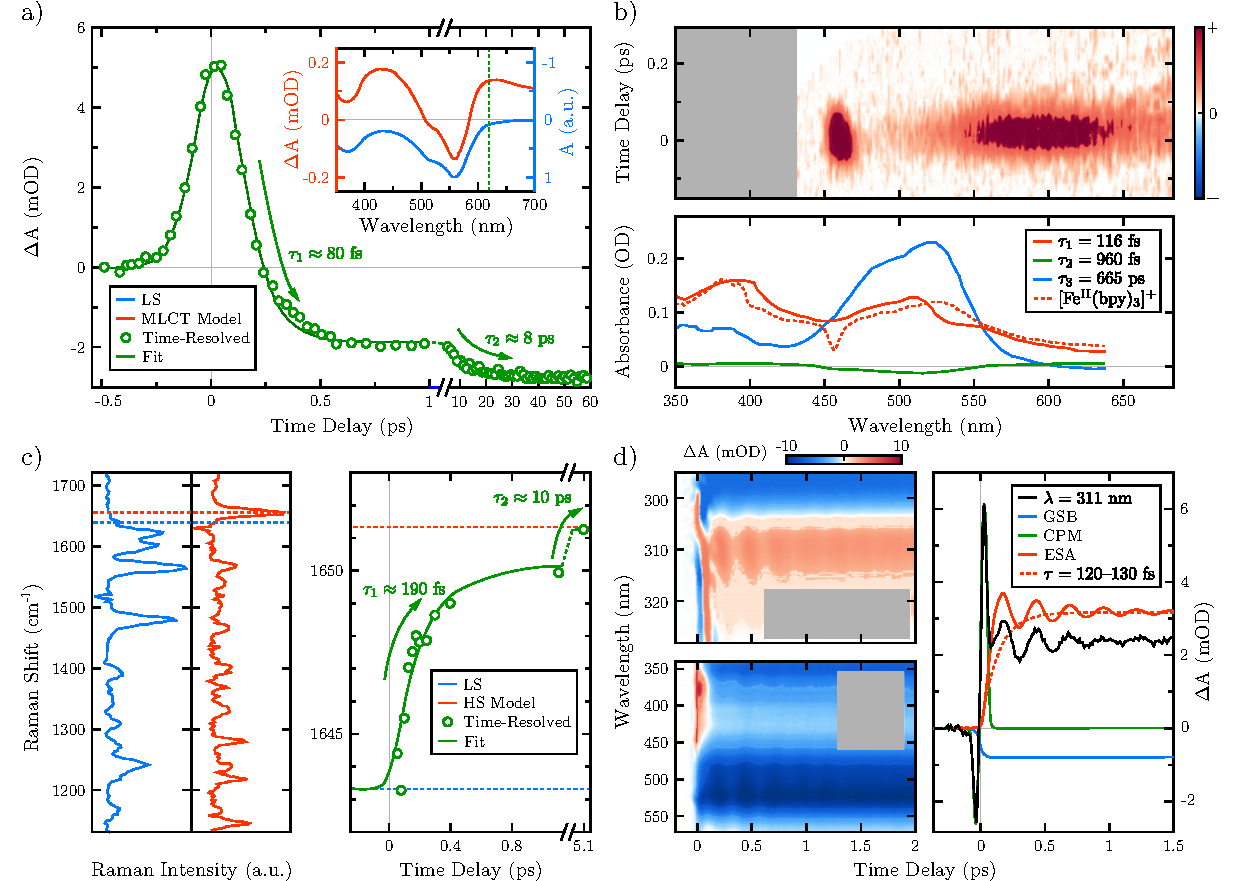
\includegraphics[width = \textwidth]{Figures/fig_SCO_literature_TA.pdf}
  \caption[Time-resolved optical measurements of photoinduced SCO.]{
    Time-resolved optical measurements of photoinduced SCO.
    (a) Single-wavelength TA scan of $\mathrm{[Fe^{II}(tren(py)_3)](PF_6)_2}$ in acetonitrile
    at $\lambda_\text{probe} = 620$~nm following 400-nm excitation;
    inset shows the absorption spectra~(blue) of LS~ground state and
    the differential absorbance~(red) of the MLCT proxy,
    i.e.~the same molecule in its reduced electrochemical state
    $\mathrm{[Fe^{II}(L)_2(L^-)]^{2+}}$.
    (b) Femtosecond FLUPS spectra~(top)
    and broadband TA decay-associated spectra~(bottom)
    of aqueous $\mathrm{[Fe^{II}(bpy)_3]^{2+}}$ under 400-nm excitation;
    the spectral feature at 466~nm is due to Raman scattering
    of the pump light by the vibrational modes of water
    ($\tilde{\nu} \approx{} 3585$~cm$^{-1}$~\cite{Harris1978}).
    (c) Steady-state Raman spectra of
    $\mathrm{[Fe^{II}}$(tren(6-\textit{H}-py)$\mathrm{_3)](PF_6)_2}$~(left, blue)
    and $\mathrm{[Fe^{II}}$(tren(6-$\mathrm{CH_3}$-py)$\mathrm{_3)](PF_6)_2}$~(right, red)
    in acetonitrile, wherein the latter is the HS proxy of the former;
    on the right side, the time evolution of the position of the spectral feature near $1650$~cm$^{-1}$
    after $560$-nm excitation of the un-methylated complex.
    (d) Broadband TA~spectra of aqueous $\mathrm{[Fe^{II}(bpy)_3]^{2+}}$
    under 580-nm excitation with UV~(top left) and Vis~(bottom left) probes;
    the $311$-nm time trace~(right, black) is shown with its fitted model components~(coloured, solid)
    and a slower 120--130-fs time profile as reported by others.
    Adapted from Refs.~\cite{Monat2000, Gawelda2007a, Smeigh2008, Aubock2015}
    respectively.
  }
  \label{fig: SCO-literature-TA}
\end{figure}

The absence of ligand-field intermediate states and an intersystem crossing
that is faster than IVR obviate the initially proposed cascade model of photoinduced SCO.
However, a direct $\mathrm{^1 MLCT} \rightarrow{} \mathrm{^5 T_{2g}}$ transition
is unlikely as well.
%
As noted by Refs.~\cite{McCusker2003, SCO-III, Juban2006},
beyond the lack of any spin--orbit coupling between
the $\mathrm{^1 MLCT}$ and $\mathrm{^5 T_{2g}}$ states~(see Tab.~\ref{tab: sco-so}),
the driving force for such a two-electron transition is expected to be
deep in the Marcus inverted region%
\footnote{Canadian chemist Rudolph A. Marcus~(1923--present) developed in 1956
a theory of electron transfer amongst molecules which predicts that
the rate constant~$k$ of such reactions do not increased monotonically with
the total Gibbs free energy~$\Delta{} G^\circ$ but
has a Gaussian dependence~\cite{Nobel1991, Marcus1993}.}
and should not give rise to a rate constant~$k = 1/\tau$ in excess of $10^{12}$~s$^{-1}$
as observed.

To check for short-lived intermediate states that could have been missed by
earlier single-wavelength TA~experiments,
Gawelda et~al~\cite{Gawelda2007a} employed
femtosecond fluorescence up-conversion spectroscopy~(FLUPS)
and broadband TA~spectroscopy (see Fig.~\ref{fig: SCO-literature-TA}b).
%
In their time-resolved emission spectra (Fig.~\ref{fig: SCO-literature-TA}b, top),
a clear signal with $\tau_1 = (20 \pm 5)$~fs is seen in the 600-nm region
where luminescence from the $\mathrm{^1 MLCT}$ state can be expected;
singular value decomposition of the broadband TA~data reveals
a spectral component which decays over $\tau_2 = (116 \pm 10)$~fs and resembles
the static absorption spectrum of the singly-reduced species of $\mathrm{[Fe^{II}(bpy)_3]^{2+}}$,
a known proxy for MLCT states.
%
Earlier studies~\cite{Damrauer1997, Yeh2000, Cannizzo2006}
into the excited-state dynamics of $\mathrm{[Ru^{II}(bpy)_3]^{2+}}$,
a transition-metal complex that is isoelectronic to $\mathrm{[Fe^{II}(bpy)_3]^{2+}}$,
have used the same techniques and
observed similar emission and absorption features that were explained by
a $\lesssim$20-fs decay of the initial $\mathrm{^1 MLCT}$ excited state
and ca.~100-fs population of the $\mathrm{^3 MLCT}$ state.%
\footnote{The evolution into the $\mathrm{^3 MLCT}$ state happens to be much more easily observable
in $\mathrm{[Ru^{II}(bpy)_3]^{2+}}$ because of its strong luminescence
and very long lifetime ($\tau = 630$~ns at $298$~K in water),
properties made possible by the fact that
$\Delta_\text{oct}(\text{Ru}) \approx 2 \Delta_\text{oct}(\text{Fe})$
for a given ligand (see Tab.~\ref{tab: cft-full} in App.~\ref{ap: cft})
and the ligand-field excited states are thus too high in energy to effectively
quench the MLCT states~\cite{Thompson2013, Hauser2017}.}
Given the correspondence between $\mathrm{[Ru^{II}(bpy)_3]^{2+}}$ and $\mathrm{[Fe^{II}(bpy)_3]^{2+}}$, similar photophysics are thought to be at work,
in the form of the two-step relaxation pathway
$\mathrm{^1 MLCT} \xrightarrow[\tau_1]{\text{IC}} \mathrm{^3 MLCT}
\xrightarrow[\tau_2]{\text{ISC}} \mathrm{^5 T_{2g}}$.
%
Support for this model is found by Smeigh et~al~\cite{Smeigh2008},
who followed indirectly followed the structural evolution of $\mathrm{[Fe^{II}(tren(bpy)_3)]^{2+}}$
using femtosecond stimulated Raman spectroscopy~(FSRS) and
recovered a time constant of $(190 \pm 50)$~fs
for the appearance of the vibrational features%
\footnote{No vibrational feature characteristic of the $\mathrm{^1 MLCT}$ state
is observed at early times in Ref.~\cite{Smeigh2008}
since it is very short-lived ($\lesssim$20~fs) and is associated
with large lifetime spectral broadening ($500$~cm$^{-1}$)~\cite{Kukura2007}.}
characteristic of the $\mathrm{^5 T_{2g}}$ state (see Fig.~\ref{fig: SCO-literature-TA}c).
%
Further evidence of an ultrafast and direct conversion from the MLCT states to the final HS state
comes from later broadband TA~measurements in the infrared~\cite{Wolf2008},
ultraviolet~\cite{Consani2009}, and visible~\cite{Tribollet2011, Cammarata2014} probe regions
with increasing temporal resolution~\cite{Aubock2015}.
%
In a recent work, shown in Fig.~\ref{fig: SCO-literature-TA}d,
Aub\"{o}ck and Chergui~\cite{Aubock2015} concluded that
the arrival into the vibrationally hot HS state should occur within $50$~fs
after the initial excitation into the $\mathrm{^1 MLCT}$ state.

%%%%%%%%%%%%%%%%%

% Experimental works
\subsection{Photoinduced Spin Crossover in X-ray Experiments}
\label{sec: SCO-photo-3}

% X-ray works - XAS, EXAFS, XANES
Concurrent to the optical measurements,
the physics of SCO and LIESST have also been intensely investigated
using different X-ray techniques ---
particularly, X-ray absorption spectroscopy~(XAS)
in steady state~\cite{Briois1995, Chen1995, Erenburg1999, Lee2000, Boca2000}
and with high temporal resolution~\cite{Bressler2004, Chen2005, Bressler2008,
Bressler2010, Cannizzo2010, Milne2014, Hong2015, Zhang2015, Chergui2016,
Gawelda2016, Chergui2017b, Collet2018a}.

% Basics of XAS
As described in Refs.~\cite{Rehr2000, deGroot2001, Glatzel2005, Chen2005, Chergui2009,
Bressler2010, Calvin2013},
X-ray photons are absorbed as electrons from orbitals deep in the atomic potential
are photoexcited to partially filled or empty higher-energy states,
i.e.~above the Fermi level $E_\text{F}$.
When the photon energy~$E_\text{X}$ is equal to or exceeds the binding energy~$E_\text{B}$,
transitions from the core to the free continuum above the vacuum level
suddenly become available,
causing absorption to increase sharply at these specific energies
and then gently decrease on the order of ${E_\text{X}}^{-3}$
as the rapidly oscillating EM field decouples from the electronic wavefunction.
%
Altogether, these features thus give the characteristic sawtooth-like appearance to
a XAS spectrum, as seen on the left side of Fig.~\ref{fig: SCO-literature-Xray}a.
On the top right side of same panel, the electronic transitions corresponding to
each absorption edge%
\footnote{The first observation of an X-ray absorption edge was made in 1913
by French experimental physicist Maurice de~Broglie (1875--1960),
the elder brother of Louis de~Broglie (see Fn.~\ref{fn: Louis_deBroglie}).
For a detailed historical account of XAS, see Refs.~\cite{Bordwehr1989, Lytle1999}.}
are shown and labeled by the X-ray term symbol of the initial state
from which the electron is ejected:
K, L$_1$, L$_2$, L$_3$ for 1s, 2s, 2p$_{1/2}$, 2p$_{3/2}$ respectively.
In the case of iron, the associated X-ray energies are
$7112$, $845$, $720$, $707$~eV~\cite{Henke1993}.
%
\begin{figure}[ht!]
  \centering
  \includegraphics[width = \textwidth]{Figures/fig_SCO_literature_Xray.pdf}
  \caption[Time-resolved X-ray measurements of photoinduced SCO.]{
    Time-resolved X-ray measurements of photoinduced SCO.
    (a) XAS~spectrum of bulk iron~(left)
    and XES~spectrum of aqueous $\mathrm{[Fe^{II}(terpy)_2]^{2+}}$~(bottom right)
    with an energy level diagram~(top right)
    showing the corresponding electronic transitions;
    the $\text{K} {\unslant[-.2] \beta}_{2,5}$ intensity is scaled up by $\times 70$;
    $\text{Val} = $ valence band, $E_\text{F} = $ Fermi level,
    $\text{QBS} = $ quasi-bound state, $\text{Vac} = $ vacuum level.
    (b) First structural characterization of the HS state of aqueous $\mathrm{[Fe^{II}(bpy)_3]^{2+}}$
    by measuring the time-dependent changes of the Fe~K-edge EXAFS~(left),
    following the reaction kinetics seen by XAS at $7126$~eV and optical TA~spectroscopy
    at $523$~nm~(top right),
    and resolving a ca.~0.20-\AA{} change in Fe--N bond length.
    (c) Femtosecond Fe~K-edge XANES measurement of aqueous $\mathrm{[Fe^{II}(bpy)_3]^{2+}}$~(left);
    time trace at $7126$~eV (top right) can be well-fitted by a simple two-step model~(bottom right).
    (d) Femtosecond Fe~L$_3$-edge XAS of $\mathrm{[Fe^{II}(tren(py)_3)]^{2+}}$ in acetonitrile~(left)
    shows a single-step $85$-fs relaxation dynamics~(right) consistent with Ref.~\cite{Smeigh2008}.
    (e) Femtosecond Fe~$\mathrm{K} \unslant[-.2]\beta_{1,3}$ XES of aqueous $\mathrm{[Fe^{II}(bpy)_3]^{2+}}$~(top left)
    is compared with XES~data from different spin-state proxies~(bottom left);
    the $7054$-eV time trace (top right) is shown with
    the best fit from two kinetics models ---
    with~(red) and without~(blue) an intermediate $\mathrm{^3 T}$ state;
    population dynamics of the former~(bottom right) is proposed.
    Panel~(a) is adapted from Refs.~\cite{Henke1993, March2017, Rehr2000};
    Panels~(b)--(f), Refs.~\cite{Henke1993, Gawelda2007b, Bressler2009, Huse2011, Zhang2014}
    respectively.
  }
  \label{fig: SCO-literature-Xray}
\end{figure}

% XAFS = EXAFS & XANES
In the XAS spectrum of condensed-phase and molecular systems,
weak oscillatory features ---
collectively referred to as X-ray absorption fine structure~(XAFS) ---
are present near and above the absorption edge
(see top left panel of Fig.~\ref{fig: SCO-literature-Xray}b and c).
%
They are modulations of the core--vacuum transition probability
caused by the interference between the photoelectron outgoing from the absorbing atom
and backscattering from other atoms nearby.
%
Depending on the energy of the photoelectron~$E = E_\text{X} - E_\text{B}$,
two regimes of XAFS exists: extended X-ray absorption fine structure~(EXAFS)
and X-ray absorption near-edge structure%
\footnote{XANES is also called NEXAFS or near-edge X-ray absorption fine structure~\cite{Bordwehr1989}.}~(XANES).

% EXAFS
The EXAFS region covers the high-energy XAS continuum above the absorption edge,
wherein $E \gtrsim 30$~eV.
In this energy regime, the photoelectron has a de~Broglie wavelength
within a typical bond length ($r_\text{Fe–N} \approx 2.0$~\AA{})
and can thus readily interfere with any part of itself
that has been singly-scattered by atoms chemically bonded to the absorber.
%
The resulting oscillations in X-ray absorption are well-described by
the `EXAFS formula'~\cite{Sayers1971, Rehr2000}:
%
\begin{equation}
  \begin{aligned}
    \chi(k) = \sum_i {S_0}^2 N_i |f_i(k)| \frac{\sin(2 k r_i + 2 \delta + \phi_i(k)) }{k r_i}
      \frac{\text{e}^{-2 r_i / L(k) }}{r_i} \text{e}^{-2 {\sigma_i}^2 k^2}
    \label{eq: EXAFS}
  \end{aligned}
\end{equation}
%
where $k = \sqrt{2 m_e E}/\hbar$ and $L(k)$ are the wavevector magnitude
and mean free path of the photoelectron,
$\chi{k}$ is the XAS spectrum after background subtraction and normalization,
$S_0$ is an overall amplitude factor;
$N_i$, $f_i = |f_i| \text{e}^{\text{i} \phi_i}$, $r_i$, and $\sigma_i$ are the coordination number, backscattering amplitude, distance, and the variance of the thermal displacement
of the $i$-th type of neighbouring atoms;
$\delta$ is the partial-wave phase shift due to the absorbing atom.%
\footnote{See Ref.~\cite{Rehr2000} for a more thorough overview on the theory of EXAFS and XANES.}
Given the similarity between this expression and Eq.~\eqref{eq: diff-int},
EXAFS is akin to electron diffraction
but highly localized in nature due to the short range of $L(k)$ and
the effect of the Debye-Waller factor $\text{e}^{-2 {\sigma_i}^2 k^2}$.
%
Indeed, by choosing $E_\text{X}$ to the edge energy of the target atom,
EXAFS can be used to directly probe the molecular structure of non-crystalline samples
with chemical selectivity, albeit only for the first few coordination shells
and without angular resolution.

% XANES
XANES refers to XAS features close to the absorption edge,
before the onset of EXAFS at $E \gtrsim 30$~eV.
%
On the `pre-edge' side, a core electron is excited to near the vacuum level
where it can occupy various empty states
(see energy diagram in Fig.~\ref{fig: SCO-literature-Xray}a),
giving rise to absorption resonances that are sensitive to
the frontier electronic structure of the absorbing atom.
%
Just above the absorption edge,
the photoelectron is ejected into free space with little kinetic energy,
where it can be backscattered by local atoms and modulate the X-ray absorption;
since its de~Broglie wavelength is much longer than the average interatomic distance,
interference of the outgoing wave is dominated by paths involving multiple scattering events
and hence the resulting modulations in X-ray absorption are highly dependent on
parameters of the local molecular geometry such as bond lengths and angles.
%
Although there is no simple quantitative treatment of XANES~\cite{Ankudinov1999, Rehr2000},
two applications --- \textsc{FEFF}~\cite{Rehr2010} and \textsc{MXAN}~\cite{Benfatto2001} ---
can be used to calculate its shape and energy.

% Ultrafast X-ray sources -> TRXAS
Given the physics of X-ray absorption, it is no surprise that XAS has been applied to study
the electronic structure of coordination complexes and the phenomenon of SCO.
Using photons with $E_\text{X}$ from $-100$ to $1000$~eV relative to
the K-edge binding energy~$E_\text{B}$ of the metal centre,
EXAFS and XANES spectra have been measured as a mean to determine
the LS and HS metal--ligand bond lengths of several Fe(II) SCO complexes
in solution~\cite{Chen1995, Hannay1997, Erenburg1999, Lee2000, Boca2000},
a feat generally unachievable by diffraction-based techniques.
%
More recently, development of X-ray sources with increasingly short pulse duration
has made it possible to deploy XAS (and XRD) in the pump-probe scheme
(see Refs.~\cite{Bressler2004, Chen2005} and the references%
\footnote{Of interest are the works in Refs.~\cite{Mills1984, Thiel1993,
Chen2001, Chen2002, Saes2003, Gawelda2005, Veen2009},
where the ms--ps photoinduced dynamics of several transition metal complexes
were probed by time-resolved XAS.} therein).

% EXAFS
Using time-resolved XAS,
Khalil, Gawelda, and co-workers~\cite{Khalil2006, Gawelda2007b}
investigated the photoinduced picosecond dynamics of three Fe(II) SCO complexes ---
$\mathrm{[Fe^{II}(tren(py)_3)]^{2+}}$, $\mathrm{[Fe^{II}(bpy)_3]^{2+}}$, and  $\mathrm{[Fe^{II}(phen)_3]^{2+}}$ --- in solution at room temperature.
From the measured differential EXAFS spectra,
they monitored the formation of the transient HS state and established that
Fe--N bond elongation also occurs during photoinduced SCO and
to the same extent --- about $0.2$ \AA{} --- as in the case of thermal SCO
(see Fig.~\ref{fig: SCO-literature-Xray}b).
Later EXAFS works~\cite{Sato2009, Nozawa2010, Canton2014, XZhang2015, Vanko2015}
in other similar systems confirm this result.

% XANES
Bressler and others~\cite{Bressler2009, Lemke2013, Cammarata2014} followed up
on these works by probing the Fe K-edge XANES region with sub-ps X-ray pulses
and monitoring absorption features which are known
proxies of the bond-elongated HS state~\cite{Hannay1997, Briois2001};
Fig.~\ref{fig: SCO-literature-Xray}c shows data that is representative of these works.
Monoexponential fitting of the time trace at $E_\text{X} = 7126$~eV indicates that
the formation of the HS photoproduct is a one-step process%
\footnote{At least within the IRF of these measurements,
which is $\tau_\text{IRF} \approx 110$--$250$~fs FWHM.}
with time constant~$\tau \approx 150$--$170$~fs,
consistent with the idea of a direct $\mathrm{^{1,3} MLCT} \rightarrow \mathrm{^5 T_{2g}}$
relaxation pathway as derived from optical TA~data (see Sec.~\ref{sec: SCO-photo-2}).
%
% L-edge XAS (Huse2010, Huse2011)
Contemporary soft X-ray measurements by Huse and others~\cite{Huse2010, Huse2011, Hong2015}
focused on the Fe L$_2$-, L$_3$-edges wherein $E_\text{B} \approx 720$, $707$~eV respectively.
XANES absorption at these energies involves Laporte-allowed%
\footnote{German-American physicist Otto Laporte (1902--1971) recognized that
electronic transitions in molecules with an inversion centre only occur if
$\Delta \ell = \pm 1$~\cite{LaporteMemoir, Laporte1925, Harris1978}.}
$\text{2p} \rightarrow \text{3d}$ transitions; they are particularly sensitive to
changes in the electronic spin state of the metal centre and the metal--ligand interaction
via selective excitation of $\mathrm{2p}_{1/2}$, $\mathrm{2p}_{3/2}$ electrons
to $\text{3d}$~vacancies, split respectively by spin--orbit coupling
and the ligand field~\cite{Briois1995}.
%
As seen in Fig.~\ref{fig: SCO-literature-Xray}d,
$\text{LS} \rightarrow \text{HS}$ conversion gives rise to a pronounced redshift to the L$_3$ edge
and transients that can be well-fitted to the same three-level
$\mathrm{^1 A_{1g}} \xrightarrow[]{h \nu} \mathrm{^{1,3} MLCT} \rightarrow \mathrm{^5 T_{2g}}$
model as before, with $\tau = (85 \pm 75)$~fs.

% XES, triplet state?
% Gaffney work~\cite{Zhang2014, Zhang2015}.
Absorption of hard X-rays leaves holes in the electronic core of the targeted atom
that are filled by electrons in higher orbitals on the sub-fs time scale,
giving rise to near-instantaneous X-ray fluorescence of comparable energy.
The right panels of Fig.~\ref{fig: SCO-literature-Xray}a show
the main observable emission peaks%
\footnote{There are two competing notations for X-ray spectral lines: Siegbahn and IUPAC.
For example, emission from transitions from the $\mathrm{M_3, M_2}$~levels to the K~level
is denoted by $\mathrm{K} \unslant[-.2] \beta_{1,3}$ or K-M$_{3,2}$~\cite{Jenkins1991}.
Note that `Siegbahn' refers to Swedish physicist Manne Siegbahn (1886--1978),
who won the 1924 Nobel Prize in Physics for his work in X-ray spectroscopy~\cite{SiegbahnMemoir}.}
associated with the K-edge ---
$\text{K} {\unslant[-.2] \alpha}$, $\text{K} {\unslant[-.2] \beta}$
from $\mathrm{1s} \rightarrow \mathrm{2p}$, $\mathrm{1s} \rightarrow \mathrm{3p3d}$ transitions respectively~\cite{deGroot2001}.
%
Vank\'{o} et~al~\cite{Vanko2006} have demonstrated that
X-ray emission spectroscopy~(XES) can be used as a sensitive probe
of the spin state of a SCO complex by quantifying the variations in
the lineshape of these emission features.
%
Since then, others~\cite{Vanko2010, Vanko2013, Haldrup2012, Haldrup2016, Miaja2016, March2017}
have employed XES in the pump--probe scheme to follow
the picosecond relaxation of the photoinduced HS state of
$\mathrm{[Fe^{II}(bpy)_3]^{2+}}$ in water.
%
Zhang et~al~\cite{Zhang2014, Zhang2015} followed up
by recording femtosecond $\text{K} {\unslant[-.2] \beta}_{1,3}$ XES spectra of this sample
in a bid to track its ultrafast excited-state spin dynamics.
%
Their data is shown in Fig.~\ref{fig: SCO-literature-Xray}e.
By comparing the time-resolved fluorescence difference spectra~(top left)
with the static ones of different spin-state proxies%
\footnote{Iron coordination complexes of different ground-state spin moments
stand in for possible excited-state spin configurations of BPY:
$\mathrm{[Fe^{III}(bpy)_3]^{3+}}$ (doublet, $S = 1/2$),
$\mathrm{[Fe^{II}Pc]}$ (triplet, $S = 1$),
$\mathrm{[Fe^{II}(phen)_2(NCS)_2]}$ (quintet, $S = 2$);
$\mathrm{Pc^{2-}}$ = phthalocyanine ($\mathrm{C_{32}H_{16}N_8}$).} (bottom left),
they confirmed the population of the $\mathrm{^5 T_{2g}}$ HS state within ca.~150~fs
after photoexcitation ($\tau_\text{IRF} = 130$--$170$~fs FWHM).
However, subtle differences in fitting (top right) led them
to suggest that SCO occurs sequentially,
in a two-step process wherein an intermediate state ---
likely a metal-centered triplet ligand-field state of type $\mathrm{^3 T}$ ---
is transiently populated;
i.e.~$\mathrm{^{1,3} MLCT} \xrightarrow[]{\tau_1} \mathrm{^3 T} \xrightarrow[]{\tau_2}
\mathrm{^5 T_{2g}}$  where $\tau_1 = (150 \pm 50)$~fs and $\tau_2 = (70 \pm 30)$~fs.
%
Indeed, this interpretation is a throwback to the early cascade model for SCO,
which is generally incompatible with the results from optical TA~spectroscopy
as discussed in Sec.~\ref{sec: SCO-photo-2} and by Brady et~al in Ref.~\cite{SCO-III}.

% Lemke 2017 paper
% structure model with distribution, 50 fs -> phase shift, damping -> triplet state
Most recently, Lemke et~al~\cite{Lemke2017} repeated their earlier XANES measurements~\cite{Lemke2013}
at a much higher temporal resolution ($\tau_\text{IRF} = (59 \pm 12)$~fs FWHM)
and also found evidence of a $\mathrm{^3 T}$ transient intermediate state
during photoinduced SCO, albeit indirectly as another source of dephasing
in their wave-packet dispersion model.
In the same vein, they reported a MLCT lifetime of $(120 \pm 10)$~fs and
claim that the previously reported $50$-fs value is a misattribution
of a phase shift caused by the convolution of the MLCT population decay
with an $265$-fs oscillation.

Finally, it is worthwhile to mention that photoinduced SCO has been investigated
using time-resolved XRD~\cite{Lorenc2009, Cailleau2010, Lorenc2012, Collet2012a,
Collet2012b, Kaszub2013, Marino2015, Freyer2013}.
%
Most of such works had picosecond--nanosecond regime and
focused on the mechanical equilibration
--- unit cell volume expansion and strain wave propagation ---
that occurs long after the formation of HS state in a solid sample.
%
A notable exception is a study by Freyer et~al~\cite{Freyer2013}
wherein a polycrystalline thin film of $\mathrm{[Fe^{II}(bpy)_3](PF_6)_2}$
is excited via two-photon absorption and then probed using $100$-fs X-ray pulses.
The resulting Debye-Scherrer diffraction patterns are used to derive
three-dimensional electron density maps at each time delay.
%
Curiously and in contrast to previous literature,
the authors reported quasi-instantaneous step-like
and unphysically large effects ---
ca.~1-\AA{} bond elongations and charge transfers of 10--30~e$^-$
from the Fe atom and $\mathrm{PF_6}^{-}$ counterions to the bipyridine ligands ---
that is explained away therein by significant delocalization
of the photoexcitation into adjacent unit cells.

% As discussed above, ultrafast structural dynamics in the form of Fe--N bond elongation
% and other coupled nuclear motions has been indirectly observed to occur concomitantly
% with the spin switching process.

% Two-photon~\cite{Castellano1997}. Review~\cite{Elsaesser2014}.

% TR XRD \cite{Lorenc2009, Collet2012a, Collet2012b, Kaszub2013, Freyer2013}.
% Freyer2013
% -> two-photon absorption from Ru(bpy) paper where 4.2 mJ/cm2 (800 nm 1050 mW at 80 MHz, 20um spot)
% ok since Ryan used ~3.3 mJ/cm2

%%%%%%%%%%%%%%%%%%%%%%

% Discuss controversy
\subsection{`Alternative Facts' of Photoinduced Spin Crossover}
\label{sec: SCO-photo-4}

From the above discussions, it is clear that the detailed mechanism
by which photoinduced SCO occurs is still an open question.

% Experiment impasse
Experimentally, the major challenge in resolving the reaction pathway is
detecting the entire excited-state dynamics with high enough temporal resolution.
%
However, each of the aforementioned pump--probe techniques has its own shortcomings.
In brief, metal--ligand MLCT states are invisible to Fe~$\text{K} {\unslant[-.2] \beta}$ XES
while triplet states are inaccessible by optical TA~spectroscopy due to the Laporte rule
and spin sensitivity is unavailable to Fe~K-edge XANES due to core-hole lifetime broadening.
%
Indeed, several authors~\cite{Hauser2017, Fatur2017, Sousa2018b, Zhang2018}
have pointed out that various studies have reported conflicting results:
the $\mathrm{^3 T}$-type states serve either as virtual coupling pathways for
bridging the $\mathrm{^{1,3} MLCT}$ and $\mathrm{^5 T_{2g}}$ states
(e.g.~Refs.~\cite{Monat2000, Bressler2009, Aubock2015}),
real intermediates that are transiently populated
(e.g.~Refs.~\cite{Cammarata2014, Zhang2014, Lemke2017, Zerdane2017}),
both (Ref.~\cite{Moguilevski2016}), or neither (Ref.~\cite{Freyer2013}).

% Peak power problem
% molar absorption coefficient of Fe(tren(py)3), Fe(terpy)2, Fe(bpy)3 in Cho2012
% Haldrup2016 SI discusses multiphoton effects
A possible explanation for the discrepancies amongst the works of different authors
could be the sample excitation condition that is used in the experiments.
For reference, the key excitation parameters --- peak pump fluence, peak pump intensity,
and surface excitation fraction --- for some studies have been calculated from given values;
they are tabulated in Tab.~\ref{tab: SCO-exc}.
%
\begin{table}[ht!]
  \centering
  {\renewcommand*{\arraystretch}{1.5}
    \begin{tabular}{ c c c c c}
      \toprule
      \multirow{2}{*}{Work} & \multirow{2}{*}{Technique}
        & \multirow{2}{*}{
          \begin{minipage}[c]{2.75cm} \centering Peak Fluence (mJ/cm$^2$) \end{minipage}}
        & \multirow{2}{*}{
         \begin{minipage}[c]{2.75cm} \centering Peak Intensity (GW/cm$^2$) \end{minipage}}
        & \multirow{2}{*}{$\eta_\text{exc}^0$} \\
        & & & & \\
      \midrule
      \cite{Gawelda2007a}  & FLUPS     & 2.8      & 71         & 0.06      \\
      \cite{Aubock2015}    & UV TA     & 0.7      & 18         & 0.01      \\
      \cite{Aubock2015}    & Vis TA    & 2.2      & 55         & 0.07      \\
      \cite{Freyer2013}    & TR-XRD    & 32       & 800        & ?         \\
      \cite{Gawelda2007b}  & XAS       & 180      & 1800       & 4.2       \\
      \cite{Zhang2014}     & XES       & 120      & 1714       & 9.4       \\
      \cite{Haldrup2016}   & XES/XDS   & 275      & 3922       & 2.1       \\
      \cite{Huse2011}      & XAS       & 3.0      & 43         & 0.4       \\
      \cite{VanKuiken2016} & XAS       & 4.2      & 42         & 0.1       \\
      \hdashline
      \cite{Field2016}     & TA        & 3.0      & 56         & 0.07      \\
      \cite{Jiang2017}     & UED       & 2.8      & 46         & 0.1       \\
      \bottomrule
    \end{tabular}
  }
  \caption{Sample excitation condition for select pump--probe works in SCO literature,
    calculated from given values.
    $\eta_\text{exc}^0$ is the excitation fraction at the surface of the sample,
    estimated to be the number of absorbed photons per pump pulse divided by
    the number of available absorbers as the optical path length~$l \to 0$.
    }
  \label{tab: SCO-exc}
\end{table}
%
By inspection, many of the X-ray works (see App.~\ref{ap: sco-exc} for a full tabulation)
excite their sample very strongly,
employing pump pulses with peak intensities on the order of 1~TW/cm$^2$.
Assuming the Beer-Lambert law and an excitation quantum yield $\Phi \approx 1$,
one can estimate the excitation fraction at the surface of the sample
to be several absorbed photons per iron centre,
condition that is ripe for various photochemical reactions beyond SCO.


Indeed, Lorenc et~al~\cite{Lorenc2009, Collet2012a, Collet2012b, Lorenc2012, Kaszub2013}
have reported that their crystalline SCO samples are visibly damaged
when $f \gtrsim 30$~mJ/cm$^2$ or $I \gtrsim 300$~GW/cm$^2$.
%
Fig.~\ref{fig: SCO-literature-alt}a shows a pump-fluence dependence measurement for
an aqueous solution of $\mathrm{[Fe^{II}(bpy)_3]^{2+}}$
and the onset of nonlinear response to photoexcitation
can be seen to begin at $80$~mJ/cm$^2$ ($1.1$~TW/cm$^2$)~\cite{Zhang2014}.
For the same sample, Lemke et~al~\cite{Lemke2017} have found somewhat higher but similar
values for nonlinearity: $220$~mJ/cm$^2$ ($4.4$~TW/cm$^2$).
%
% Figure of Zhang2014, original vs corrected, fluence and intensity x-scale
% Note that Tarnovsky2006 unit of sigma mistake
\begin{figure}[ht!]
  \centering
  \includegraphics[width = \textwidth]{Figures/fig_SCO_literature_alt.pdf}
  \caption[Alternative facts of photoinduced SCO.]{
    Alternative facts of photoinduced SCO.
    (a) Dependence of the change in sample transmission~$\Delta T$~(left)
    and absorbance~$\Delta A$~(right) as a function of the peak fluence/intensity
    of the pump laser pulse for $\mathrm{[Fe^{II}(bpy)_3]^{2+}}$ in water.
    (b) Photochemistry of aqueous $\mathrm{[Ru^{II}(bpy)_3]^{2+}}$
    under intense femtosecond laser excitation;
    absorption spectrum~(left) and transient concentration~(right)
    of different photoproducts:
    GND = $\mathrm{[Ru^{II}(bpy)_3]^{2+}}$ (ground state),
    $\mathrm{^3 MLCT}$ = $\mathrm{[Ru^{III}(bpy^-)(bpy)_2]^{2+}}$ (targeted excited state),
    Red = $\mathrm{[Ru^{II}(bpy^{\cdot -})(bpy)_2]^{+}}$ (reduced ion),
    Ox = $\mathrm{[Ru^{III}(bpy)_3]^{3+}}$ (oxidized ion),
    $\mathrm{e^{-}_{aq}}$ = solvated electrons.
    (c) Adiabatic calculations suggest two possible ISC pathways --- sequential~(red)
    and direct~(blue) --- depending on whether the spin--orbit coupling
    is taken to the first or second order and whether structural distortions
    are included.
    (d) Alternate modeling of SCO based on vibronic relaxation supports
    direct and very fast conversion to the $\mathrm{^5 T_{2g}}$ state.
    Panels~(a), (b), and (d) are adapted from Refs.~\cite{Zhang2014, Tarnovsky2006, Chang2010};
    Panels~(b)--(f), Refs.~\cite{Sousa2013, Sousa2018b} respectively.
  }
  \label{fig: SCO-literature-alt}
\end{figure}
%
In the SCO works of the present thesis (see Secs.~\ref{sec: TA-BPY} and \ref{sec: UED-AZA}),
the $100$-nm thick crystal samples start to degrade
at $> 1.4$~mJ/cm$^2$ ($23$~GW/cm$^2$) and exhibit immediate irreversible damage
at $> 10$~mJ/cm$^2$ ($200$~GW/cm$^2$).
%
Therefore, conclusions from works involving terawatt-level photoexcitation
ought to be assessed with caution since any subtle changes in spectral shape,
some of which have been assigned to intermediate spin states~\cite{Zhang2014} or
large-scale charge transfers and delocalization~\cite{Freyer2013},
could simply be artifacts from undesirable photoproducts generated by multiphoton processes acting
on the SCO complex and its spectators (e.g.~counterions and solvent molecules).
%
Notably, many works could not be evaluate as easily in this light
since their respective authors did not state the value of either the peak fluence
and intensity of the pump pulse directly or all the parameters%
\footnote{Wavelength~$\lambda$, beamwidth~$w$ on the sample, pulse duration~$\tau$,
and energy~$E$ (see App.~\ref{ap: sco-exc}).} necessary to calculate them.
%
Similarly, few included the absorption spectrum of the sample in non-arbitrary units
that is necessary for an estimate of the excitation fraction~$\eta_\text{exc}$.

% Explanation from X-ray people
In Refs.~\cite{Tarnovsky2006, Haldrup2016, Biasin2016},
the effect of intense photoexcitation on $\mathrm{[Ru^{II}(bpy)_3]^{2+}}$ in water
are discussed with respect to XAS and XES experiments.
%
As seen in Fig.~\ref{fig: SCO-literature-alt}b,
pumping of the $\mathrm{^1 MLCT}$ band at 40--170~mJ/cm$^2$ (0.3--1.3~TW/cm$^2$)
drives multiphoton processes and generates significant population of several photoproducts.%
\footnote{Four species could be spectrally resolved:
solvated electrons $\mathrm{e^-}_\text{aq}$,
the $\mathrm{^3 MLCT}$ excited state $\mathrm{[Ru^{III}(bpy)_2(bpy^{-})]^{2+}}$
the reduced ion $\mathrm{[Ru^{II}(bpy)_2(bpy^{\cdot -})]^+}$,
and the oxidized ion $\mathrm{[Ru^{III}(bpy)_3]^{3+}}$.}
Nevertheless, it is argued that the transient analysis of data from such experiments
continues to be justified since the SCO gateway state, $\mathrm{^3 MLCT}$,
remains as the dominant species ($> 66$~\%) and
the photochemistry of this $\mathrm{Ru^{II}N_6}$ complex could be analogous to
that of $\mathrm{[Fe(bpy)_3]^{2+}}$ and $\mathrm{[Co(terpy)_3]^{2+}}$.
%
Possibly in response to this issue,
two recent XANES works~\cite{Zhang2017, Kjaer2017} have opted for
unusually low excitation conditions, $0.1$~mJ/cm$^2$ ($2$~GW/cm$^2$)
or one absorbed photon for every ca.~300 iron centre~(!)
while another persisted and used $1.28$--$3.85$~TW/cm$^2$~(\textinterrobang)~\cite{Kong2019}.


% Theory side
Given the ambiguity on the experimental side,
one could be expected to seek guidance from theory.
Numerous theoretical studies have investigated the photoinduced SCO process
by means of several approaches~\cite{Koshino1999, Ordejon2008, deGraaf2010, Sousa2013,
Domingo2014, Sousa2017, Sousa2018a, Sousa2018b, Vanko2015, Suaud2009, Iuchi2014, Iuchi2016,
Veeneedaal2010, Chang2010, Veenendaal2017, Nance2015, Kuiken2011, Capano2013,
Papai2013, Fredin2014, Penfold2018}.
Unfortunately, there is no consensus therein either.
%
Some works find that a direct $\mathrm{^3 MLCT} \rightarrow \mathrm{^5 T_{2g}}$ pathway is
unlikely at first~\cite{Ordejon2008, deGraaf2010, Sousa2013, Domingo2014, Sousa2017}
but becomes feasible when second-order spin--orbit coupling and structural distortions
are included~\cite{Sousa2018a, Sousa2018b}.
Fig.~\ref{fig: SCO-literature-alt}c summarizes the two different proposed
mechanisms (red = sequential, blue = direct);
the right panels show the values of $\mathrm{^3 MLCT}$ lifetime
that could be generated from a collection of 16 structural conformations
along a molecular dynamics~(MD) trajectory of a $\mathrm{[Fe^{II}(bpy)_3]^{2+}}$ molecule
in water at 300~K.
%
Others~\cite{Veeneedaal2010, Chang2010, Veenendaal2017} could describe
extremely fast ISC events wholly within the $\mathrm{^{1,3,5} MLCT}$ manifold,
bypassing any $\mathrm{^3 T}$ transient intermediate state,
by invoking vibronic dissipation to prevent recurrence of the initial state
and leakage back to the $\mathrm{^1 A_{1g}}$ state (see Fig.~\ref{fig: SCO-literature-alt}d).
%
Alternatively, McCusker and Hauser~\cite{McCusker2014, Hauser2017} have
questioned the validity of intermediate states whose lifetimes are less than
a single vibrational period along the reaction coordinate;
instead, they have mused about a vibronic wave packet coherently relaxing
down a barrierless hypersurface of mixed singlet--quintet and metal--ligand character.

With impasses on both the experimental and theoretical fronts,
such is the present thinking on the exact pathway of photoinduced SCO.

% 0.003 A EXAFS \cite{Liu2017}

% Solvated electron discussion in Tarvosky et al (2006), a Chergui paper on Ru(bpy)

% Comparison of d-MLCT and d-d/LF excitation \cite{Zerdane2017}

% iron photosensitizer record~\cite{Harlang2015, Chabera2017, Chen2018}.
% Long lived MLCT states~\cite{Liu2016, Shepard2016, Chabera2017}

% Review on light/ligand-induced type SCO \cite{Chastanet2018}.

% Cooperativity in crystals, vanishing in metal-diluted systems.
% sign of cooperativity:
% 1) sigmoidal shape of curve,
% 2) shift of 1A1->3T1 absorption band by 200 cm-1 during 1A1 ground state recovery

% Practical application~\cite{Kahn1992, Krober1993}.

%%%%%%%%%%%%%%%%%%%%%%%%%%%%%%%%%%%%%%%%%%

% SCO in Fe(bpy)3
\section[Spectral Signatures of Spin Crossover in \protect{[Fe\textsuperscript{II}(bpy)\textsubscript{3}](PF\textsubscript{6})\textsubscript{2}}]{Spectral Signatures of Spin Crossover in \\ \protect{[Fe\textsuperscript{II}(bpy)\textsubscript{3}](PF\textsubscript{6})\textsubscript{2}}}
\label{sec: TA-BPY}

% intro
Tris(2,2'-bipyridine)iron(II) $\mathrm{[Fe^{II}(bpy)_3]^{2+}}$
and other transition-metal polypyridyl complexes have been
extensively studied~\cite{Hauser2017, McCusker2019}.
%
First reported in 1888, interest in these molecules was driven initially
by their use as colorful and chemically stable redox indicators:
red for iron(II) and blue for iron(III)~\cite{Brandt1954}.
%
Later, it was found that a long-lived, catalytically active,
and strongly luminescent triplet state ($\mathrm{^3 MLCT}$)
can be created in $\mathrm{[Ru^{II}(bpy)_3]^{2+}}$ and
$\mathrm{[Os^{II}(bpy)_3]^{2+}}$ quickly and efficiently
after exposure to visible light~\cite{Thompson2013}.
%
As such, $\mathrm{[Fe^{II}(bpy)_3]^{2+}}$ was studied mostly
as an isoelectronic~(d$^6$) homologue~\cite{Chen2018, Wenger2018}
with a more earth-abundant and less-expensive metal centre
for practical applications such as dye-sensitized solar cells
and organic light-emitting diodes~\cite{Weber2013, Ponseca2017, Bizzarri2018}.
%
As in the case of Ru and Os, this complex also has MLCT intermediate states
with significant ligand-centered electron density (see Fig.~\ref{fig: BPY-intro})
that is available for injection into the conduction band of a nearby electron acceptor.
%
Since then, a vast body of work has been published
detailing its photophysical properties.
%
\begin{figure}[t!]
  \centering
  \includegraphics[width = \textwidth]{Figures/fig_BPY_intro.pdf}
  \caption[Electron spin density difference of different excited states.]{
    Electron spin density difference $(\rho_\alpha - \rho_\beta)$
    of different excited states:
    (a) $\mathrm{^3 T_{1g}}$ (an extra $\alpha$~e$^-$ on metal);
    (b) $\mathrm{^5 T_{2g}}$ (two extra $\alpha$~e$^-$ on the metal);
    (c) $\mathrm{^1 MLCT}$ (an extra $\alpha$~e$^-$ on the metal
    and an extra $\beta$ e$^-$ on the ligand);
    (d) $\mathrm{^3 MLCT}$ (two extra $\alpha$~e$^-$ on both sites);
    Adapted with permission from Refs.~\cite{Sousa2013, Zhang2018}.
  }
  \label{fig: BPY-intro}
\end{figure}

% LIESST in BPY
Discovery of LIESST brought renewed focus on the $\mathrm{[Fe^{II}(bpy)_3]^{2+}}$ complex
as it has been shown to readily undergo the ultrafast and highly efficient photoinduced SCO process
that is discussed in the previous sections of this thesis chapter.
%
In particular, unlike many other SCO molecules with a $\mathrm{Fe^{II} N_6}$ coordination sphere,
there is no thermally driven $\text{LS} \rightarrow \text{HS}$ transition%
\footnote{
From kinetic considerations (Eq.~\eqref{eq: kHL-lowT}),
a LS---HS equilibrium temperature of $\mathrm{[Fe^{II}(bpy)_3]^{2+}}$
can be estimated to be ca.~700~K;
however, it is purely theoretical since the molecule would have
thermochemically dissociated already~\cite{SCO-II}.}
in this molecule that could be inadvertently triggered by laser-deposited heat
and be mistaken for the light-induced process.
%
As such, it has become the prototypical sample for
time-resolved pump--probe experiments studying
the early-time excited-state dynamics of this class of molecular systems,
as is the case herein.

% Although chemical similarity, this molecule does not readily luminesce
% and various close polypyridyl derivatives
% --- e.g.~$\mathrm{[Fe^{II}(terpy)_2]^{2+}}$ and $\mathrm{[Fe^{II}(tren(py)_3)_3]^{2+}}$ ---
% have been prepared to manipulate the vary the relative energy between different MOs.


% Chergui2012: almost instantaneous vibrational cooling? Stoke shift fluorescence at t~0 fs.

% M-polypyridine, M(bpy), M = Ru
% Compare Fe(tren(py)), Fe(terpy), Fe(bpy)? See Cho2012.

% HOMO, LUMO diagrams in VanKuiken2016
% Structure of Fe(tren(py), Fe(terpy), Fe(bpy) in Cho2012


% Recent paper: \cite{Carey2019}

% Ru(bpy)3 big TA paper \cite{Damrauer1997}

% Association with Ru(bpy)3, more abundant and cheaper but fast relaxation by intermediates
% weaker delta -> metal-centered LF states are lower in energy than MLCT states -> short MLCT time
% Destabilize ligand-field states to stabilize MLCT state

% Big review on Ru(bpy)3, \cite{Thompson2013}

% Electronic spectra of M(bpy)3, M = Cu, Ni, Co, Fe, Ru
% Palmer and Piper, Inorg. Chem. 1965


% UV spectra of M(bpy)3, M = Mn, Fe, Co, Ni, Cu, Zn
% Xu, Smith, Weber. Inorg. Chem. 2016

% Phosphoresence spectra of M(bpy)3, M = Zn, Ru, Os, Rh
% \cite{Nozaki2006}


% Decomposition of MLCT overlap with LF bands. See figure 6 of Domingo2014.

% Application with earth abundant metal bpy~\cite{Weber2013, Bizzarri2018, Wenger2018}.

% Figure: MO structures (VanKuiken2016), MLCT bands (Domingo), absorption vs fluorescence

\subsection{Methods}

% figure:  photo of sample, crystal structure of BPY
\begin{figure}[ht!]
  \centering
  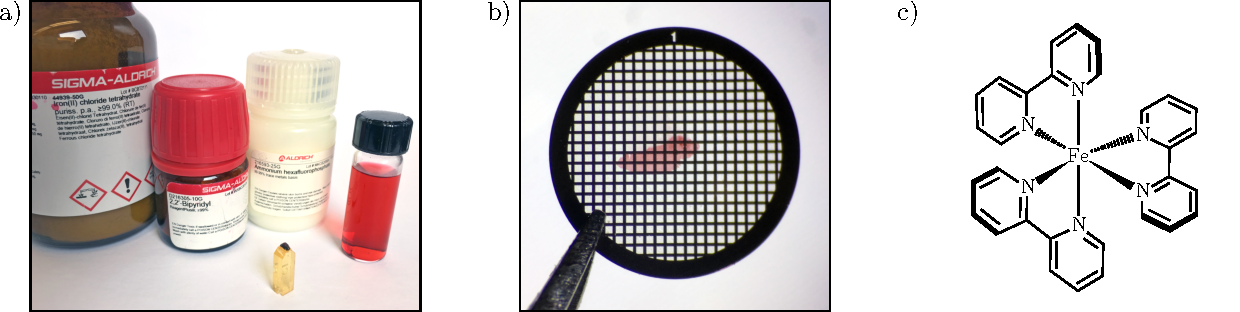
\includegraphics[width = \textwidth]{Figures/fig_BPY_photo.pdf}
  \caption[Photos of BPY sample.]{
    Photos of BPY sample:
    (a) reagents for synthesis~(left),
    a vial of aqueous BPY solution~(right),
    and a singular crystal of BPY embedded on a block of epoxy~(centre);
    (b) 200-nm thick crystal section mounted on a TEM~mesh
    as view under an optical microscope;
    (c) molecular structure of $\mathrm{[Fe^{II}(bpy)_3]^{2+}}$.
  }
  \label{fig: BPY-photo}
\end{figure}

% first time with fs TA in single crystal
Here, the ultrafast photophysics of $\mathrm{[Fe^{II}(bpy)_3]^{2+}}$
is revisited using femtosecond UV--Vis broadband TA~spectroscopy.
Unlike all previous studies where the complex is dissolved in acetonitrile or water,
the present work is a study in the single-crystal phase.

% Sample prep
Two compounds are synthesized: $\mathrm{[Fe^{II}(bpy)_3]Cl_2}$ and
$\mathrm{[Fe^{II}(bpy)_3](PF_6)_2}$.
For the former, 2,2'-bipyridine is dissolved in acetonitrile and then added to
an aqueous solution of $\mathrm{Fe^{II} Cl_2}$;
the mixture is gently heated to $70^{\circ}$~C, stirred for two hours,
filtered, dried under vacuum, and re-crystallized in acetonitrile.
The $\mathrm{PF_6^-}$ salt is prepared by counterion exchange:
the previously prepared $\mathrm{[Fe^{II}(bpy)_3]Cl_2}$ is dissolved in water
and added to an aqueous solution of $\mathrm{NH_4PF_6}$;
the mixture is stirred at room temperature for 30 minutes;
$\mathrm{[Fe^{II}(bpy)_3](PF_6)_2}$ forms as a dark red precipitate which is
collected by filtration, dried in the air, and re-crystallized in acetonitrile
(see Fig.~\ref{fig: BPY-photo}).

% microtome
Single-crystal samples of $\mathrm{[Fe^{II}(bpy)_3](PF_6)_2}$ of varying thickness
(ca.~100--300~nm) are prepared by ultramicrotomy:
slices are cleaved along the $(210)$ crystal plane and loaded onto 0.5-mm thick sapphire%
\footnote{Sapphire is chosen here for its high thermal conductivity,
which allows laser-deposited heat to dissipate in between laser shots.} substrates.
Unless otherwise noted, a sample thickness of $200$~nm is used for
all single-crystal TA~measurements.
Solution-phase samples are also prepared and measured for reference:
$\mathrm{[Fe^{II}(bpy)_3]Cl_2}$ is dissolved in deionized water and
probed in a flow cell with $150$-$\unslant\mu$m thick quartz windows
and 400-$\unslant\mu$m optical path length;
The flow rate is ca.~0.42~mL/s, sufficient to ensure a new target for each laser shot.

% Experimental setup
The experimental setup that is used for this work is described in Sec.~\ref{sec: TA-setup}
and was designed and built by Dr.~Ryan L. Field as part of his doctoral project~\cite{Ryan-thesis}.
%
400-nm, 53-fs pump pulses are used for sample excitation.
They are generated by frequency doubling the 800-nm, 40-fs fundamental of the laser.
%
The broadband supercontinuum probe pulses (Fig.~\ref{fig: BPY-data-whitelight})
are generated by WLG.
For the measurements in the visible spectrum,
a small fraction of the $800$-nm fundamental of the laser
is circularly polarized using a quarter-wave plate and then focused into
a 2-mm thick $\mathrm{CaF_2}$ plate that is kept under constant rotation to prevent damage.
The output beam is collimated and returned to linear polarization
using an achromatic quarter-wave plate;
residual seed light is removed using an optical filter.
%
For the UV measurements, the fundamental is first frequency-doubled by SHG
before an equivalent WLG~setup wherein some of the optics are replaced
with UV-appropriate ones.

% white-light spectrum (UV, VIS)
\begin{figure}[t!]
  \centering
  \includegraphics[width = \textwidth]{Figures/fig_BPY_data_whitelight.pdf}
  \caption[Typical spectrum of the UV and Vis supercontinuum probes.]{
    Typical spectrum of the supercontinuum probes
    used in the UV and visible measurements,
    produced via WLG pumped by 400-nm~(dashed line)
    and 800-nm light~(solid line).
    The IRF width as a function of probe wavelength
    is also shown.
    Adapted from Ref.~\cite{Ryan-thesis} with permission from Dr.~Ryan L. Field.
  }
  \label{fig: BPY-data-whitelight}
\end{figure}

% pump, probe condition
At the sample position, the pump and probe beams are focused to a $1/\mathrm{e}^2$~diameter
of about 90~$\unslant\mu$m and 60~$\unslant\mu$m respectively,
using all-reflective optics to avoid additional laser chirp.
The pump fluence is generally ca.~3.3~mJ/cm$^2$, corresponding to a pulse energy of 100~nJ
and peak intensity of $62$~GW/cm$^2$, well within the regime of linear response.
%
The probe polarization is set to maximize the main absorption feature of the sample at 533~nm
while the pump polarization is set to either $0^\circ$ for the single-crystal measurements
or the `magic angle'%
\footnote{Absorption of an isotropic sample after photoexcitation is given by
$\Delta A(t, \beta) \propto N(t) [ 1 + (3 \cos^2 \beta - 1) R(t) ]$,
where $N(t)$, $R(t)$, and $\beta$ are respectively the excited-state population,
the alignment of the transition dipoles, and the relative pump--probe polarization angle.
Setting $\beta = \arccos \frac{1}{\sqrt{3}}$ eliminates the contribution
of dipole-alignment relaxation~\cite{FlemingBook}.}
(ca.~54.7$^\circ$) for those in solution.
%
The IRF time is estimated to be approximately $(80 \pm 9)$~fs and $(90 \pm 11)$~fs FWHM
in the UV and visible ranges respectively.
%
The time delay between pump and probe pulses is set using a motorized translation stage
with a minimum travel of 100~nm (ca.~0.7~fs).

For each time point, each `pump-on' and `pump-off' spectrum is integrated over
four consecutive probe pulses and averaged 200~times.
Along the wavelength axis, the data is also smoothed by a moving average
over five adjacent entries, corresponding to a range of ca.~0.7~nm.
%
The magnitude of the TA~spectra is normalized against variations in pump laser intensity
that is measured from a weak reflection using a slow photodiode.

Data analysis of the TA~spectra has been described in detail in Sec.~\ref{sec: TA-data-analysis}.


\subsection{Experimental Results}

Fig.~\ref{fig: BPY-data-linabs} shows the measured linear absorption spectra of
both solvated and single-crystal BPY at room temperature
using the UV and Vis supercontinuum probes.
By inspection, they are consistent with previously reported results
in solution~\cite{Yamasaki1937, Williams1955, Schlafer1956, Creutz1980,
Gawelda2007a, Consani2009, Zhang2014, Aubock2015, Carey2019}
and crystals~\cite{Palmer1966, Felix1979, Decurtins1980, Ferguson1982b}.
%
From Refs.~\cite{Ceulemans1981, Kober1982, Ferguson1982a, Ferguson1983, Domingo2014},
the broad absorption bands in the Vis range are assigned to
$\text{d}\unslant[-.2]\pi \rightarrow \text{L}\unslant[-.2]\pi^*$ electronic transitions
from the ground state~($\mathrm{^1A_{1g}}$) to the MLCT manifold~($\mathrm{^{1, 3, 5}MLCT}$).
The strong UV peaks are due to
$\text{L}\unslant[-.2]\pi \rightarrow \text{L}\unslant[-.2]\pi^*$ transitions
within the 2,2'-bipyridine ligands.

% Figure: Absorption spectrum of aqueous and single-crystal Fe(bpy)
\begin{figure}[ht!]
  \centering
  \includegraphics[width = \textwidth]{Figures/fig_BPY_data_linabs.pdf}
  \caption[Absorption spectrum of single-crystal and solvated BPY.]{
    Absorption spectrum of single-crystal and solvated BPY,
    as measured using the UV~(dashed line) and Vis~(solid line) probe.
    Adapted with permission from Ref.~\cite{Ryan-thesis}.
  }
  \label{fig: BPY-data-linabs}
\end{figure}

% Difference between solution and crystal spectra
There are some notable differences between the measured solution and single-crystal
absorption spectra.
%
For one, the features of the latter are significantly narrower,
likely resulting from less homogeneous and inhomogeneous broadening at work
in the static environment of the crystal.
%
There are also variations in the relative magnitude of the absorption peaks
which can be similarly explained by the different degrees of freedom
available to the BPY molecules in either media.
In particular, the polarization of the probe light is fixed in relation to the sample
whilst the molecules and their transition dipole moments are either also fixed
--- as in the case of the crystal --- or constantly tumbling in all orientations otherwise.

% Figure: Fluence dependence
\begin{figure}[ht!]
  \centering
  \includegraphics[width = \textwidth]{Figures/fig_BPY_data_fluence.pdf}
  \caption[Fluence dependence of single-crystal BPY.]{
    Fluence dependence of the TA spectrum of solvated and single-crystal BPY at $t = +5$~ps.
    Inset: linear trendlines at three select probe wavelengths
    (cyan $= 313$~nm, magenta $= 489$~nm, black $= 533$~nm).
  }
  \label{fig: BPY-data-fluence}
\end{figure}

Fig.~\ref{fig: BPY-data-fluence} shows the UV--Vis TA~spectrum at $t = +5$~ps of single-crystal BPY
as a function of peak laser fluence of the pump pulse.
From the trendlines in the insets,
it is clear that BPY exhibits a linear response to $400$-nm laser excitation
for peak fluences up to $10$~mJ/cm$^2$ or peak intensities of ca.~200~GW/cm$^2$.
%
Few-shot and irreversible changes to the absorption spectrum of
single-crystal samples and notable distortions of the transmitted pump and probe beams
are observed to occur immediately above this regime,
indicating that the damage threshold had been reached.
%
No equivalent threshold for the solution samples could be reached
since the quartz windows of the flow cell itself became visible damaged
towards the upper reaches of the fluence range.


%%%%%%%%%%%%%%%%%

% Aqueous data

In addition to the control experiment that is the above measurements on fluence dependence,
a full TA~dataset of solvated BPY has been have collected such it can be directly compared
with previous solution-phase studies, particularly Refs.~\cite{Gawelda2007a, Consani2009, Aubock2015}.
%
To cover adequately the temporal and spectral range of
the excited-state dynamics present in BPY,
the dataset was taken over four separate ways:
a short $5$-ps scan in steps of $10$ fs and
a long $900$-ps one in steps of $2$ ps,
once using the UV probe and another with the Vis probe.
%
After some data preprocessing in the form of windowing and artifact removal,
these scans become the data that is shown in the four panels of Fig.~\ref{fig: BPY-data-aqueous}.

% Figure: UV-Vis TA data of aqueous Fe(bpy)
\begin{figure}[ht!]
  \centering
  \includegraphics[width = \textwidth]{Figures/fig_BPY_data_aqueous.pdf}
  \caption[UV--Vis TA~spectra of solvated BPY.]{
    UV--Vis TA~spectra of solvated BPY after artifact removal.
  }
  \label{fig: BPY-data-aqueous}
\end{figure}

% Describe data
By inspection, several features can be immediately seen in the TA~spectra of solvated BPY.
In addition to the strong CPM~signal around time-zero,
there is the GSB that spans most of the UV--Vis spectrum and decays over several hundred picoseconds.
%
There are also two ESA: a short-lived one localized near $420$~nm
and another at $\lesssim$335~nm that narrows or shifts deeper into the UV spectrum
and persists for as long-lived as the GSB.
%
Some fast oscillations are discernible in the short-time scans
under the GSB and the long-lived ESA.

% Global analysis
To disentangle the various spectral components in the TA~data and quantify
their temporal evolution, global analysis is applied.
%
As described in Sec.~\ref{sec: TA-data-analysis},
each of the four data matrices are diagonalized by SVD and
reduced to their principal basis spectra and kinetic traces,
i.e.~the left and right singular vectors associated with the largest singular values.%
\footnote{See Fig.~\ref{fig: BPY-data-aqueous-svd} in App.~\ref{ap: sco-bpy}
for plots of these principal components.}
%
These kinetic traces are then globally fitted to a decay model composed of
a few exponential functions convolved with a Gaussian IRF
while the basis spectra are transformed into their corresponding DAS.

% Figure: aqueous global fit + residuals
\begin{figure}[t!]
  \centering
  \includegraphics[width = \textwidth]{Figures/fig_BPY_data_aqueous_resi.pdf}
  \caption[Global analysis of solvated BPY TA~data.]{
    Global analysis of solvated $\mathrm{[Fe^{II}(bpy)_3](PF_6)_2}$ TA~data:
    (a) UV short-time, (b) UV long-time, (c) Vis short-time, (d) Vis long-time.
    From left to right, the panels show
    the GA fit, GA fit residuals, and SVD~truncation residuals respectively.
  }
  \label{fig: BPY-data-aqueous-resi}
\end{figure}
%
In Fig.~\ref{fig: BPY-data-aqueous-resi},
the results of the global analysis are shown:
the fitted exponential spectral components~(left),
the fit residuals containing the non-exponential features~(centre),
and the noisy SVD~truncation residuals~(right).
%
Indeed, the exponential and oscillatory dynamics of the data
have been neatly separately from the noise which is mostly caused by
fluctuations in the intensity of the pump and probe pulses;
they can now be examined independently.

% Figure: aqueous DAS
\begin{figure}[t!]
  \centering
  \includegraphics[width = \textwidth]{Figures/fig_BPY_data_aqueous_DAS.pdf}
  \caption[Decay-associated spectra of solvated BPY.]{
    Decay-associated spectra of solvated BPY:
    UV short-time, UV long-time, Vis short-time, and Vis long-time
    (from left to right, top to bottom).
  }
  \label{fig: BPY-data-aqueous-DAS}
\end{figure}
%
Fig.~\ref{fig: BPY-data-aqueous-DAS} shows
the decay-associated spectra~(DAS) of solvated BPY
in the same arrangement as the TA~data from which they are derived.

In the long-time data, there is effectively a single exponential component:
$\tau \approx (645 \pm 6)$--$(699 \pm 12)$~ps.
In both the UV and visible region, this component has the same spectral profile as
the linear absorption spectrum of ground-state BPY (see Fig.~\ref{fig: BPY-data-linabs}).
As such, they simply reflect the repopulation of the $\mathrm{^1 A_{1g}}$ LS state
which comes at the end of photoinduced SCO process.

% Figure: aqueous frequency analysis
\begin{figure}[t!]
  \centering
  \includegraphics[width = \textwidth]{Figures/fig_BPY_data_aqueous_Welch.pdf}
  \caption[Frequency analysis of solvated BPY short-time TA~data.]{
    Frequency analysis of solvated BPY short-time TA~data:
    (a) power spectrum of the GA fit residuals as a function of probe wavelength,
    (b) cross section at $\tilde{\nu} = 128$~cm$^{-1}$ (dashed line on the left panels).
  }
  \label{fig: BPY-data-aqueous-Welch}
\end{figure}

In the short-time data, there are three exponential components:
$\tau_1 \approx (62 \pm 29)$--$(86 \pm 5)$~fs, $\tau_2 \rightarrow \infty$,
and $\tau_3 \rightarrow \infty$.
%
The $\tau_1$ component has a IRF-limited lifetime that is comparable to
that of some DAS ($116$ fs and $56$ fs) of Refs.~\cite{Gawelda2007a, Aubock2015} respectively.
As in these previous works, the profile of this short-time component,
which contains the fleeting ESA near $425$~nm, is consistent with the linear absorption spectrum
of reduced BPY or $\mathrm{[Fe^{II}(bpy)_3]^+}$,
a known proxy for the $\mathrm{^3 MLCT}$ excited state
that forms shortly after photoexcitation.
Therefore, it is herein assigned to the decay of the initially excited $\mathrm{MLCT}$ state
to the $\mathrm{^5 T_{2g}}$ HS state.
%
The $\tau_3$ component corresponds to the ca.~650-ps $\text{LS} \leftarrow \text{HS}$
relaxation process which would appear as a GSB with an effectively infinite lifetime
on this time scale.
%
Lastly, there is the intermediate $\tau_2$ component that is absent in the visible spectrum.
Given that its profile resembles that of the first derivative of the $\tau_3$ component,
it is interpreted to be a manifestation of the spectral narrowing and shifting expected
of a HS state that is dissipating a large amount of excess energy into its surrounding.
%
Support for this interpretation is found in Refs.~\cite{Consani2009, Lemke2017}
wherein similar time constants --- $(1.6 \pm 0.1)$, $(1.14 \pm 0.17)$, $(3.4 \pm 1.2)$~ps ---
were described and assigned to vibrational cooling of
the newly formed and very `hot' $\mathrm{^5 T_{2g}}$ HS state.

% aqueous frequency analysis
By inspection of the fit residuals of the short-time TA~data
(Fig.~\ref{fig: BPY-data-aqueous-resi}),
clear oscillations can be seen under both the ESA and GSB~features
in the UV and visible regions.
%
To evaluate their distribution as a function of probe wavelength,
Welch's method~\cite{Welch1967} is applied to each individual time trace of the TA~data.
%
In the resulting 2D~power spectrum (Fig.~\ref{fig: BPY-data-aqueous-Welch}),
a single $(128 \pm 13)$~cm$^{-1}$ mode is apparent, strongly in the UV region
and weakly in the visible one, with a spectral profile that is consistent
with the linear absorption spectrum of the ground state.
%
This observation has been reported before~\cite{Consani2009, Aubock2015}
and it was assigned to a coherent vibrational wavepacket on the potential energy surface of
the $\mathrm{^5 T_{2g}}$~state along either an N--Fe--N bending mode,
a Fe--N stretching mode, or a combination of both.

%%%%%%%%%%%%%%%%%%

% Single-crystal data

% Figure: UV-Vis TA data of single-crystal Fe(bpy)
\begin{figure}[t!]
  \centering
  \includegraphics[width = \textwidth]{Figures/fig_BPY_data_crystal.pdf}
  \caption[UV--Vis TA~spectra of single-crystal BPY.]{
    UV--Vis TA~spectra of single-crystal BPY after artifact removal.
  }
  \label{fig: BPY-data-crystal}
\end{figure}
%
Fig.~\ref{fig: BPY-data-crystal} shows a full TA~dataset of single-crystal BPY,
collected in the same manner as for aqueous BPY:
a short- and long-time scan in both the UV and visible regions.
Note that more of the UV spectrum could be sampled herein
since the $\text{L}\unslant[-.2]\pi \rightarrow \text{L}\unslant[-.2]\pi^*$ transitions
are weaker%
\footnote{Caveat: depending on the relative polarization of the probe.}
in single-crystal BPY, allowing enough of the supercontinuum probe
to transmit through the sample and reach the detector.

% Figure: single-crystal SVD + global fit results
\begin{figure}[t!]
  \centering
  \includegraphics[width = \textwidth]{Figures/fig_BPY_data_crystal_resi.pdf}
  \caption[Global analysis of single-crystal BPY TA~data.]{
    Global analysis of single-crystal BPY TA~data:
    (a) UV short-time, (b) UV long-time, (c) Vis short-time, (d) Vis long-time.
    From left to right, the panels show
    the GA fit, GA fit residuals, and SVD truncation residuals respectively.
  }
  \label{fig: BPY-data-crystal-resi}
\end{figure}
%
% Global fitting
Again, global analysis as per Sec.~\ref{sec: TA-data-analysis}
is applied to suppress the uncorrelated noise and extract the principal exponential components
of the dynamics.%
\footnote{See Fig.~\ref{fig: BPY-data-crystal-svd} in App.~\ref{ap: sco-bpy}
for plots of the principal components.} The results are shown in
Fig.~\ref{fig: BPY-data-crystal-resi}.
%
Notably, as seen in the GA fit residuals,
there are many more and stronger oscillatory features herein than in the case of solvated BPY.

% Figure: crystal DAS
\begin{figure}[t!]
  \centering
  \includegraphics[width = \textwidth]{Figures/fig_BPY_data_crystal_DAS.pdf}
  \caption[Decay-associated spectra of single-crystal BPY.]{
    Decay-associated spectra of single-crystal BPY:
    UV short-time, UV long-time, Vis short-time, and Vis long-time
    (from left to right, top to bottom).
  }
  \label{fig: BPY-data-crystal-DAS}
\end{figure}
%
Fig.~\ref{fig: BPY-data-crystal-DAS} shows the DAS of the single-crystal BPY data,
as generated from the GA fit.
%
In the long time scale, there are two exponential components in both the UV and
visible regions of the spectrum: $\tau_1 = (98 \pm 1)$--$(100 \pm 3)$~ps
and $\tau_2 \rightarrow \infty$.
%
As seen in Fig.~\ref{fig: BPY-data-crystal-DAS-GSA},
the spectral profile of the $\tau_1$ component can be matched readily
with the linear absorption spectrum of ground-state BPY.
%
This suggests that the $\text{LS} \leftarrow \text{HS}$ ground-state recovery of BPY
occurs much faster in the single-crystal environment than in solution.
%
In addition, there is the $\tau_2$~component that is not observed in
the long-time TA~data of solvated BPY.
By inspection, its spectral profile bears a strong resemblance to
the second derivative%
\footnote{To avoid noise, GSA'' is evaluated numerically
by calculating the double finite difference of not the measured GSA values directly
but an analytical approximation generated by Voigt fitting~\cite{Abrarov2011}.}
of the linear absorption spectrum of ground-state BPY
and acts to broaden its absorption peaks.
%
As reported before by others~\cite{Colvin1993, Farztdinov1997},
this lineshape can be interpreted to be the result of the Stark~effect%
\footnote{Johannes Stark (1874--1919) found that an external electric field
can shift the spectral lines of an atom by coupling with its electric dipole moment;
for this discovery, he was awarded the 1919 Nobel Prize in Physics~\cite{Nobel1901}.}
involving random electric fields generated by laser-induced heating
of the crystal lattice.

% Figure: crystal DAS vs GSA
\begin{figure}[t!]
  \centering
  \includegraphics[width = \textwidth]{Figures/fig_BPY_data_crystal_DAS_GSA.pdf}
  \caption[Comparison between the long-time DAS and the GSA of single-crystal BPY.]{
    Comparison between the long-time decay-associated spectrum~(DAS) and
    the ground state absorption~(GSA) of single-crystal BPY.
    GSA'' refers to the second derivative of the latter.
  }
  \label{fig: BPY-data-crystal-DAS-GSA}
\end{figure}

% Short-time DAS
At the short time scale, there are three exponential components:
$\tau_1 = (72 \pm 6)$--$(108 \pm 13)$~fs, $\tau_2 = (1.7 \pm 0.4)$~ps,
and $\tau_3 \rightarrow \infty$.
%
The first component has a lifetime and spectral profile that is consistent
with those derived for one of the short-time solution DAS.
Thus, it assigned as before to the decay of the initially excited MLCT state into the HS state.
%
Similarly, the $\tau_2$ and $\tau_3$ components correspond respectively
to the vibrational cooling of the HS state and its conversion back to the LS ground state.

% Figure: crystal frequency analysis (short-time)
\begin{figure}[ht!]
  \centering
  \includegraphics[width = \textwidth]{Figures/fig_BPY_data_crystal_Welch.pdf}
  \caption[Frequency analysis of single-crystal BPY short-time TA~data.]{
    Frequency analysis of single-crystal BPY short-time TA~data:
    (a) power spectral density of the GA fit residuals as a function of probe wavelength,
    (b) cross sections at select wavenumbers~$\tilde{\nu}$
    (dashed lines on the left panels).
  }
  \label{fig: BPY-data-crystal-Welch}
\end{figure}

Now that the exponential features of the principal components have been resolved,
frequency analysis is performed on the residuals that are left over after subtracting the GA fits
(centre panels of Fig.~\ref{fig: BPY-data-crystal-resi}).
The short-time results are shown in Fig.~\ref{fig: BPY-data-crystal-Welch}
where four modes are readily discernible:
$(55 \pm 7)$, $(81 \pm 7)$, $(139 \pm 11)$, and $(165 \pm 7)$~cm$^{-1}$.
%
These oscillations are likely to be related to vibrational modes of the BPY molecule.
However, assignment is difficult since the uncertainty of the extracted wavenumber values is
relatively large and there are few studies that have focused on vibrational spectroscopy of BPY
in the single-crystal environment.

% Figure: TA data with different OD,
\begin{figure}[ht!]
  \centering
  \includegraphics[width = \textwidth]{Figures/fig_BPY_data_crystal_OD.pdf}
  \caption[UV--Vis TA~spectra of single-crystal BPY with different sample thickness.]{
    UV--Vis TA~spectra of single-crystal BPY
    with different sample thickness, as measured by absorbance at $533$~nm:
    $0.33$, $0.62$, $0.97$, $1.12$~OD (from left to right, top to bottom).
  }
  \label{fig: BPY-data-crystal-OD}
\end{figure}

On the longer time scale, oscillations with periods on the order of hundreds of picoseconds
are visible. Similar features have been readily observed in UED traces of nanometre-thick
single-crystal films; they are indicative of coherent acoustic phonons generated by
laser-induced thermoelastic deformation of the crystal lattice~\cite{Harb2009, Gao2013, Jiang2017}.
%
To verify this assertion within TA~spectroscopy,
long-time scans were collected from single-crystal BPY samples
of different absorbances (and therefore thicknesses), as prepared by ultramicrotomy.
%
Indeed, as seen in Fig.~\ref{fig: BPY-data-crystal-OD}, the period of these slow oscillations
expectedly increases with sample absorbance.
%
More precisely, frequency analysis of these long-time scans shows a single mode
whose period varies varies linearly with sample absorbance
along a slope of $190$~ps/OD (Fig.~\ref{fig: BPY-data-crystal-Welch-lon}).
%
This correlation is consistent with an acoustic phonon that is propagating
with a speed of sound of $2.7$~km/s through a solid with
an Young's modulus of $12.6$~GPa whilst subject to the boundary conditions
defined by the crystal thickness.%
\footnote{$v = \frac{1}{c \epsilon}(\frac{\Delta T}{\Delta A})$,
where $v$ is the speed of sound, $\frac{\Delta T}{\Delta A}$ is the period/absorbance linear slope,
$c = 2.13$~M and $\epsilon = 9160$~{M$^{-1}$ cm$^{-1}$} are the molar concentration
and absorptivity at $533$~nm of single-crystal BPY;
$B = \rho v^2$, where $B$ and $\rho = 1.73$~g/cm$^3$ are its bulk modulus and density.}
Indeed, others~\cite{Shepherd2012, Hernandez2014, Felix2015} have reported similar values
for the speed of sound and Young's modulus of several related SCO nanoparticles using
techniques such as high-pressure XRD, atomic force microscopy, and nuclear inelastic scattering.
%
Furthermore, the spectral profile of this mode matches that of the first derivative
of the ground state absorption ($|\text{GSA}'|$),
confirming that it is a displacive feature which modulates the relative energy of the electronic states.
%
Generally, this type of behaviour is not observed in solid-state systems nor
any other without cryogenic cooling; very narrow absorption lineshapes are necessary
to resolve the minute variations in energy levels~\cite{Nelson1982, Miller1984}.
%
Given the readily discernible acoustic oscillations in the long-time TA~scans herein,
it is inferred that there is exceptional strong electron--phonon coupling in single-crystal BPY.

% Figure: crystal frequency analysis (long-time)
\begin{figure}[t!]
  \centering
  \includegraphics[width = \textwidth]{Figures/fig_BPY_data_crystal_Welch_lon.pdf}
  \caption[Frequency analysis of single-crystal BPY long-time TA~data.]{
    Frequency analysis of single-crystal BPY long-time TA~data ($A = 0.97$~OD):
    (a) power spectrum of the GA fit residuals as a function of probe wavelength,
    (b) cross section at $\tilde{\nu} = 0.18$~cm$^{-1}$,
    (c) linear trend between the absorbance~$A$ and
    the long-time oscillation period~$T = \frac{1}{c \tilde{\nu}}$
    for different samples.

  }
  \label{fig: BPY-data-crystal-Welch-lon}
\end{figure}


\subsection{Discussions}

% Short-time dynamics between solvated and single-crystal BPY
The TA~spectra of solvated and single-crystal BPY in the present work
are imminently comparable in terms of early-time exponential features.

% Figure: short-time DAS for aqueous and crystal
\begin{figure}[ht!]
  \centering
  \includegraphics[width = \textwidth]{Figures/fig_BPY_data_DAS_sho.pdf}
  \caption[Short-time decay-associated spectra of solvated and single-crystal BPY.]{
    Short-time decay-associated spectra of (a) solvated and (b) single-crystal BPY.
  }
  \label{fig: BPY-data-DAS-sho}
\end{figure}

Fig.~\ref{fig: BPY-data-DAS-sho} shows the DAS extracted from the short-time part
of these datasets.
%
Given the similar spectral profiles and time constants,
it appears that BPY exhibits the same decay process under both chemical environments.
%
Considering the assignment in the previous section,
photoinduced SCO in BPY occurs via an extremely fast ($\lesssim$100~fs) decay
from one of the $\mathrm{MLCT}$ state directly onto
the HS potential energy surface where there is vibrational cooling
on the order of ca.~2~ps and eventual relaxation back to the LS ground state.
%
In particular, contrary to the interpretation of Ref.~\cite{Freyer2013},
the electronic dynamics in single-crystal BPY is evidently confined to
the Fe~centre and three bpy~ligands of a single complex
in the first few picoseconds.
%
Any significant delocalization of the initial photoexcitation ---
e.g.~charge transfer to the $\mathrm{PF_6^-}$ counterions or neighbouring unexcited BPY complexes ---
should give rise to observable spectral and fluence-dependent differences
between the photoresponse of the single-crystal and solution samples.
%
Indeed, there was none detected in this study or those of others working on
related SCO systems~\cite{Tissot2011, Lorenc2012, Collet2012a, Collet2012b, Bertoni2016a, Bertoni2016b}.
%
Similarly, no collective spin transition ($\Phi > 1$)
was seen within the measured time scale of the experiment nor expected
since the laser-induced heating and compression necessary to
overcome the LS--HS equilibrium in BPY are much higher than
its damage threshold~\cite{SCO-II}.


% Short-time oscillations
Assignment of the various oscillations that are discernible
in the power spectrum of the short-time TA~data (Figs.~\ref{fig: BPY-data-aqueous-Welch}
and \ref{fig: BPY-data-crystal-Welch}) is ambiguous due to their limited temporal sampling
and a lack of consistent vibrational studies of BPY in the literature.
%
Conveniently, Aub\"{o}ck and Chergui~\cite{Aubock2015} have compiled
all the low-frequency ($< 200$~cm$^{-1}$) vibrational modes that have been reported
on BPY and the closely related complex $\mathrm{[Fe^{II}(phen)_2(NCS)_2]}$.
%
In particular, one DFT~work~\cite{Alexander2008} predicted in~vacuo
the four similarly-valued modes --- $61$, $86$, $140$, $163$~cm$^{-1}$ ---
corresponding respectively to a combination of N--Fe--N stretching and chelate twisting,
degenerate out-of-plane motion of the bipyridine ligands, and two types of Fe--N stretching.
%
Another theoretical work reported several modes in the LS state ---
$144.6$, $170.2$~cm$^{-1}$ (Fe--N stretching) --- and the HS state ---
$132.7$, $149.6$, $152.4$~cm$^{-1}$ (N--Fe--N bending) ---
that are within the margin of error of the present observations.
%
Experimentally, Consani and Aub\"{o}ck~\cite{Consani2009, Aubock2015}
have found only three modes --- $127$, $157$, $225$~cm$^{-1}$ --- in their UV TA~measurement
of solvated BPY and they were assigned ambiguously to vibrational wavepackets
involving some combination of Fe--N stretching and N--Fe--N bending.
%
IR and Raman measurements of solid-state $\mathrm{[Fe^{II}(phen)_2(NCS)_2]}$
in Ref.~\cite{Ronayne2006} yielded a number of low-frequency vibrational modes,
among which include three in the LS state --- $81$, $139$, $163$~cm$^{-1}$ ---
and two in the HS state --- $131$, $133$~cm$^{-1}$ --- that overlap with those herein.
%
In Ref.~\cite{Cammarata2014}, femtosecond optical TA~in single crystals of the same molecule
showed evidence of coherent vibrations at $85$~cm$^{-1}$ and $113$~cm$^{-1}$
which were assigned respectively to a ligand butterfly-like bending mode
and a totally symmetric Fe--N stretching mode of the HS state.

Given the present observations and those in the above literature,
the short-time oscillations herein are most probably caused by
impulsively stimulated Raman scattering, involving vibrational modes on
the LS potential energy surface.
%
This follows from superior quantitative agreement between our measured wavenumber values ---
$(55 \pm 7)$, $(81 \pm 7)$, $(139 \pm 11)$, and $(165 \pm 7)$~cm$^{-1}$ ---
and those reported in the LS state of BPY and $\mathrm{[Fe^{II}(phen)_2(NCS)_2]}$.
%
In addition, as seen in Figs.~\ref{fig: BPY-data-aqueous-Welch}b
and \ref{fig: BPY-data-crystal-Welch}b,
the spectral profiles of these oscillations generally match that
of the ground state absorption, suggesting that they are coupled to
the electronic transitions of the LS~state.
%
The extra modes that are activated in the SCO dynamics of single-crystal BPY
could be a consequence of denser molecular packing in the crystal environment,
wherein the single Fe--N stretch in solvated BPY becomes mixed
with some N--Fe--N bending and ligand distortions.
%
Alternatively, given the margin of error of the observed oscillations,
some of them could be vibrational modes of the HS state.
In that case, it would expected such excitations to be delayed
due to the time scale of the $\text{LS} \rightarrow \text{HS}$ transition;
such a time delay may be observable as a phase shift relative
to those oscillations which are due to impulsively stimulated Raman scattering.
%
At present, a subtle phase shift could be observed between the 81-cm$^{-1}$
and the 139-cm$^{-1}$ modes. However, it is not clearly resolved
due to the concurrent presence of 165-cm$^{-1}$ mode in this spectral region.

% Long-time dynamics
% - Broadening feature
% - Long-time decay with different time constants (chemical pressure effect)
On the longer time scale, the effects of the lattice are manifest
on the observed dynamics of single-crystal BPY.
%
Firstly, the crystal dataset shows a persistent line-broadening feature
that is effectively infinite on the order of one nanosecond.
As described previously, this is caused by thermalization of the absorbed laser energy
into the lattice. The absence of an equivalent feature in the solution data
suggests that this heat can be rapidly dissipated into the solvent bath
surrounding the excited BPY molecules.
%
Secondly, the lifetime of the HS~state in that environment was found to be nearly 100~ps,
an order of magnitude shorter than that in solution~(ca.~670~ps).
While the latter case is in line with reported values in the literature,%
\footnote{In some older works~\cite{Kirk1976, Creutz1980},
much longer lifetimes --- $(810 \pm 70)$, $(830 \pm 70)$~ps ---
were described under similar conditions (aqueous BPY at room temperature).}
which ranged from $650$~ps to $676$~ps~\cite{McCusker1992, Gawelda2007a, Consani2009},
the former has not been observed prior to the present work.
%
Here, it is proposed that this phenomenon is caused by the chemical pressure
of the greater crystal environment acting on the few solitary photogenerated HS~molecules
which would have become volumetrically endowed%
\footnote{See Fn.~\ref{fn: volume-contraction}.} by their longer Fe--N bonds.
%
In a manner analogous to the effect of applied external pressure
in the Clapeyron relation (see Sec.~\ref{sec: SCO-theory}),
the zero-point energy difference between the HS and LS states, $\Delta E_\text{HL}^{(0)}$,
increases, destabilizing the HS state and thus hastening its decay back to the LS state.

% Figure: kHL vs temperature and unit cell volume
\begin{figure}[t!]
  \centering
  \includegraphics[width = \textwidth]{Figures/fig_BPY_hostlattice.pdf}
  \caption[$\text{LS} \leftarrow \text{HS}$ relaxation rate constant of
    BPY doped in $\mathrm{[M^{II}(bpy)_3](PF_6)_2}$ single crystals.]{
    $\text{LS} \leftarrow \text{HS}$ relaxation rate constant of
    BPY doped in $\mathrm{[M^{II}(bpy)_3](PF_6)_2}$ single crystals,
    where $\text{M} = \{ \text{Co, Zn, Mn, Cd} \}$
    and the molar doping fraction is ca.~1~\%,
    as a function of
    (a) temperature and
    (b) unit cell volume of the undoped host at room temperature.
    Adapted with permission from Ref.\cite{Schenker1998}.
  }
  \label{fig: BPY-hostlattice}
\end{figure}

Supporting evidence of this description is found
in the $\text{LS} \leftarrow \text{HS}$ relaxation rate constants of
BPY doped into a series of isostructural and photophysically inert host lattices
of the form $\mathrm{[M^{II}(bpy)_3](PF_6)_2}$,
where $\text{M} = \{ \text{Co, Zn, Mn, Cd} \}$,
as measured by Schenker et~al~\cite{Schenker1998}.
%
As shown in Fig.~\ref{fig: BPY-hostlattice},
the rate of the LS recovery exponentially increases
as the unit cell volume of the host lattice decreases,%
\footnote{Note that there is a gross mismatch between the volume values
in Tab.~1 of Ref.~\cite{Schenker1998} and those plotted in all subsequent referencing figures
(e.g.~Refs.~\cite{Hauser2002, Hauser2004, SCO-II, Hauser2006}).}
suggesting that the driving force for this relaxation process becomes stronger
as the cavities in which the guest BPY molecules reside shrink~\cite{Hauser2004, Hauser2006}.
%
Similar acceleration in the $\text{LS} \leftarrow \text{HS}$ transition
has been observed in other dilute mixed crystals such as
$\mathrm{[Fe^{II}}_x \mathrm{M^{II}}_{1 - x} \mathrm{(terpy)_3] (PF_6)_2}$~\cite{Hauser2006}
and $\mathrm{[Fe^{II}}_x \mathrm{M^{II}}_{1 - x} \mathrm{(phen)_3] (ClO_4)_2}$~\cite{Bode1980}.
%
Given that the equivalent unit cell volume of BPY is significantly smaller than
those of the given host lattices ($2342$~\AA{}$^3$ versus ca.~2520--2570~\AA{}$^3$),%
\footnote{In App.~\ref{ap: cif}, the unit cell volume of BPY is given as $1561.4$~\AA{}$^3$
from Ref.~\cite{Dick1998}. The present value is calculated for an unit cell
that has undergone a coordinate transformation
($\boldsymbol{a}_3 \rightarrow \frac{3}{2}  \boldsymbol{a}_3$)
to match the one in Ref.~\cite{Schenker1998}.}
it is therefore reasonable to attribute the shortened HS lifetime observed in single-crystal BPY
to the chemical pressure effect of its own lattice.

\subsection{Summary and Conclusions}

In this work, I have characterized the ultrafast dynamics of $\mathrm{[Fe^{II}(bpy)_3](PF_6)_2}$
single crystals in the UV and visible ranges using femtosecond transient absorption spectroscopy
at low excitation fluence.

At early times, the exponential dynamics and spectral features were found
to be fully analogous to those observed previously in solvated $\mathrm{[Fe^{II}(bpy)_3]^{2+}}$.
%
This is evidence that there are few if any excitonic or collective excitations
even within the confines of a undiluted single crystal.
As others have reported in related SCO crystals~\cite{Tissot2011, Lorenc2012, Collet2012a,
Collet2012b, Bertoni2016a, Bertoni2016b, Marino2016},
the photophysics of SCO in solids, as in solution,
is purely localized to the single molecules that have been photoexcited,
contrary to the many-body interpretations described in the XRD work of Ref.~\cite{Freyer2013}.
%
Therefore, ultrafast single-crystal SCO studies as in the present work do provide
an excellent model system for probing the $\text{MLCT}$ state and the process by which
this molecular charge redistribution can apparently lead to such exceptionally fast
$\Delta S = 2$ spin transition.

Many fast oscillations were observed in the short-time single-crystal measurements
while only one can be seen in the solution data.
%
Frequency analysis showed that the spectral profiles of the former
match that of the ground state absorption and their wavenumber values are in good agreement
with those reported in literature for low-frequency vibrational modes of the LS state.
As such, these oscillations in the single crystal are most likely
impulsively stimulated Raman modes on the potential energy surface of the LS ground state.
%
On the other hand, the single mode in the solution phase corresponds more closely
to a wavepacket on the HS surface, involving either a Fe--N stretch
or N--Fe--N bend vibrational mode.

Interestingly, slow and displacive oscillations were also seen in
the long-time single-crystal dataset but not in the solution one.
Further measurements on samples of different thicknesses showed that
they are coherent acoustic waves driven by laser-induced distortions
of the crystal lattice, the same ones as seen in UED experiments
of other samples~\cite{Harb2009, Gao2013, Jiang2017}.
%
That they are readily discernible in the present optical work
suggests very strong electron--phonon coupling in this molecular system.
%
Indeed, this is the first such observation of which I am aware.
Since the publication of this work, others~\cite{Parpiiev2017}
have also detected similar acoustic waves using optical transient reflectivity spectroscopy
in single crystals of [Fe\textsuperscript{II}(PM-AzA)\textsubscript{2}(NCS)\textsubscript{2}].

% Collet paper on Fe(phen) lattice phonons~\cite{Collet2019b}.


%%%%%%%%%%%%%%%%%%%%%%%%%%%%%%%%%%%%%%%%%%

% SCO in Fe(PM-AzA)2(NCS)2
\section[Structural Dynamics of Spin Crossover in \protect{[Fe\textsuperscript{II}(PM-AzA)\textsubscript{2}(NCS)\textsubscript{2}]}]{Structural Dynamics of Spin Crossover in \\ \protect{[Fe\textsuperscript{II}(PM-AzA)\textsubscript{2}(NCS)\textsubscript{2}]}}
\label{sec: UED-AZA}


% Figure:  AZA and relatives, structures and XHS vs T
\begin{figure}[ht!]
  \centering
  \includegraphics[width = \textwidth]{Figures/fig_AZA_intro.pdf}
  \caption[Spin crossover in $\mathrm{[Fe^{II}(PM-L)_2 (NCS)_2]}$ complexes.]{
    Spin crossover in $\mathrm{[Fe^{II}(PM-L)_2 (NCS)_2]}$ complexes:
    (a) molecular structure and
    (b) HS molar fraction~$\gamma_\text{HS}$ as a function of temperature~$T$
    of powder samples at standard ambient pressure.
    Abbreviations:
    PM = \textit{N}-(2'-pyridylmethylene),
    DMA = 2,6-dimethylaniline,
    A = aniline,
    AzA = 4-(phenylazo)aniline,
    BiA = 4-aminobiphenyl,
    PEA = 4-(phenylethylnyl)aniline.
    Adapted with permission from Refs.~\cite{Ksenofontov1998, Capes2000}.
  }
  \label{fig: AZA-intro}
\end{figure}

% Intro to AZA
The focus of this section is the molecule
[Fe\textsuperscript{II}(PM-AzA)\textsubscript{2}(NCS)\textsubscript{2}] or AZA.%
\footnote{\textit{cis}-bis(isothiocyanato)bis[(\textit{N}-2'-pyridylmethylene)-
4-(phenylazo)aniline]iron(II)}
It is part of a family of transition metal complexes
that are formed by coordinating $\mathrm{Fe^{2+}}$ with a pair of
isothiocyanate~($\mathrm{NCS^-}$) and Schiff-base diimine ligands.%
\footnote{A Schiff base --- named after German-Italian chemist Hugo Schiff~(1834--1915) ---
is a molecule that is formed by reacting an amine (R--NH$_2$) with an aldehyde (R--(CO)--H)
or a ketone (R--(CO)--R'); a diimine is a compound with two imine (R,R'--C=N--R'')
groups~\cite{Schiff1864, Halcrow2007}.}
%
Barth and others~\cite{Barth1972, Konig1974, Maeda1976} originally synthesized them
to investigate their potential for thermal SCO,
given their similarity to the well-known SCO systems $\mathrm{[Fe^{II}(phen)_2(NCS)_2]}$ and
$\mathrm{[Fe^{II}(bpy)_2(NCS)_2]}$~\cite{Baker1964}.
%
As seen in Fig.~\ref{fig: AZA-intro},
distal changes to the substituents of the coordinating ligands can give rise to
the whole range of SCO behaviour:
none, incomplete, gradual, abrupt, and hysteretic~\cite{Ksenofontov1998, Guionneau1999,
Letard1999, Capes2000}.
%
The latter is the most desirable type of phase transition for practical applications
since both states are stable and addressable within a broad range of temperature
in the hysteresis loop~\cite{Kahn1992, Kumar2017, Collet2018b}.
%
AZA itself undergoes a gradual $\text{LS} \leftrightarrow \text{HS}$ thermal spin transition
at 184~K and LIESST below 44~K under the standard ambient pressure~\cite{Letard1999, Capes2000}.
%
In the interest of understanding the structure--function relationship in SCO materials,
this molecule is often treated as the non-abrupt and non-hysteretic prototype
to which other more complex systems are compared~\cite{Boillot2002, Hayami2003,
Blundell2004, SCO-II, LeGrand2008, Kepenekian2009, Guionneau2012, Guionneau2014,
XZhang2015a, Mebs2015, Lakhloufi2016, Lakhloufi2018, Hamouda2018}.
%
Systematic studies on temperature and pressure dependence
of the crystallographic and photomagnetic properties of AZA and its relatives
have shown that their physics can be well described by the Slichter-Drickamer model~\cite{Slichter1972},
%
\begin{equation}
  \begin{aligned}
    \ln \left( \frac{1 - \gamma_\text{HS}}{\gamma_\text{HS} - \gamma_\text{HS}^0} \right)
      & = \frac{\Delta H_{HL}}{RT} - \frac{\Delta S_{HL}}{R}
        + \frac{\Gamma}{RT}\left( 1 + \gamma_\text{HS}^0 - 2 \gamma_\text{HS} \right)
    \label{eq: Slichter}
  \end{aligned}
\end{equation}
%
where $\gamma_\text{HS}$ is the molar HS fraction,
$\gamma_\text{HS}^0 = \gamma_\text{HS}(T \rightarrow 0)$,
$\Delta H_{HL}$ and $\Delta H_{HL}$ are the enthalpy and entropy change between the HS and LS states,
$\Gamma$ is a parameter quantifying the strength of the interaction
between the individual molecules of the crystal lattice~\cite{SCO-III}.
%
In particular, the progression of SCO transitions --- gradual, abrupt, hysteretic ---
is recovered when the value of $\Gamma$ goes from being less than to greater than $2 R T_{1/2}$,
in increasing order of molecular interactions~\cite{Capes2000, Hayami2003,
Marchivie2003, Marchivie2005, Kepenekian2009}.

% Figure:  AZA data from Marino2016
\begin{figure}[t!]
  \centering
  \includegraphics[width = \textwidth]{Figures/fig_AZA_review.pdf}
  \caption[Static and time-resolved measurements of AZA.]{
    Static and time-resolved measurements of AZA:
    (a) optical reflectivity as a function of temperature;
    (b) thermal SCO and LIESST characterized
    by magnetic susceptibility~(top), total optical reflectivity~(middle),
    and XANES at 7125~eV~(bottom);
    (c) femtosecond optical reflectivity spectroscopy;
    (d) near-IR TA spectroscopy;
    (e) femtosecond XANES.
    Adapted with permission from Ref.~\cite{Marino2016}.
  }
  \label{fig: AZA-review}
\end{figure}

% Figure: photoinduced dynamics of AZA
% Marino2013, Marino2016, Parpiiev2017
AZA has also been the focus of three studies~\cite{Marino2013, Marino2016, Parpiiev2017}
investigating the other mystery of SCO:
the ultrafast electronic and structural dynamics that follows photoexcitation
and converts the molecule from the $\mathrm{^1 A_{1g}}$ LS~state
to the $\mathrm{^5 T_{2g}}$ HS~state.
%
It was demonstrated that changes in the optical reflectivity of AZA single crystals
are correlated with their thermal SCO transition and can thus be used to monitor
the dynamics of the photoinduced process in the pump--probe scheme
(Fig.~\ref{fig: AZA-review}a and b).
%
Indeed, fitting of time traces at select probe wavelengths (Fig.~\ref{fig: AZA-review}c)
indicated that the photocycle in AZA is similar to that in BPY and other SCO systems:
an intermediate state --- unlike either the LS and HS states, probably $\mathrm{^{1,3}MLCT}$ ---
forms and decays within 50~fs ($\tau_\text{IRF} = 80$~fs~FWHM) of photoexcitation%
\footnote{Several pump wavelengths have been used to induce SCO in AZA:
400~nm\cite{Parpiiev2017}, 647.1--676.4~nm~\cite{Letard1999, Capes2000},
800~nm~\cite{Marino2016, Jiang2017}, 830~nm~\cite{Marino2016}, and 850~nm~\cite{Marino2013}.}
of the MLCT band, followed by 500--2000~fs of vibrational cooling.
%
In Ref.~\cite{Marino2016}, femtosecond Fe~K-edge XANES and near-IR~TA spectroscopies
(Fig.~\ref{fig: AZA-review}d and e) were also applied to determine
the structure and bonding of the FeN$_6$ core of AZA
and track the formation of the HS state in real time.
%
From the exponential and oscillatory features observed therein,
it was asserted that the photoinduced SCO in AZA does proceed in two distinct steps
and vibrational cooling of the newly formed `hot' HS molecules later activates
an optical lattice phonon which eventually gives rise to further lattice dynamics,
including acoustic waves on the time scale of 100~ps~\cite{Parpiiev2017}.
%
More details could be found in the doctoral theses in
Refs.~\cite{Hoefer-thesis, Marino-thesis, Parpiiev-thesis};
in particular, Ref.~\cite{Hoefer-thesis} shows the calculated and measured far- and mid-IR spectra
of AZA in the LS and HS state and of the PM-AZA ligand by itself for comparison.

Altogether, it appears that the idea of structure--function correlation
in thermal SCO transition is also relevant to understanding the dynamics of the photoinduced process
via intra- and intermolecular couplings.
However, there is a lack of direct structural studies on the femtosecond time scale in this field.
%
Here, in a follow-up of the works described in Sec.~\ref{sec: TA-BPY},
the results of a UED measurement on AZA are presented.

% Co and Zn analogues of Fe(PM-L)2(NCS)2 \cite{Guionneau2002, LeGac2008, Guionneau2012}.

% Variable temperture XAS study of AZA~\cite{Zhang2015}.
% Temperature movie of AZA~\cite{Lakhloufi2016}.
% Fatigability of AZA~\cite{Guionneau2012}.

% Thermal hysteresis loop theory
% Theoretical prediction of a charge-transfer phase transition
% Hiroko Tokoro, Asuka Namai, Marie Yoshikiyo, Rei Fujiwara, Kouji Chiba & Shin-ichi Ohkoshi
% Scientific Reports volume 8, Article number: 63 (2018)

\subsection{Methods}

% Figure: Photos of AZA samples
\begin{figure}[ht!]
  \centering
  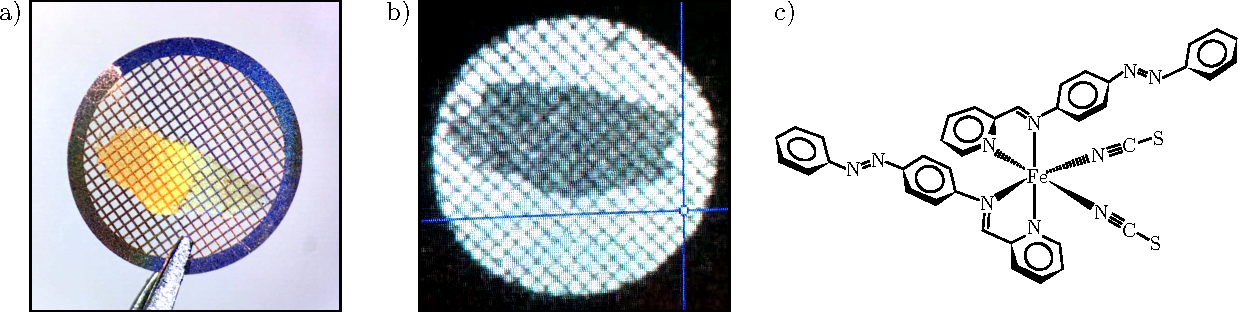
\includegraphics[width = \textwidth]{Figures/fig_AZA_photo.pdf}
  \caption[Photos of AZA sample.]{
    Photos of a 100-nm thick AZA sample mounted on a TEM mesh
    and illuminated by (a) visible light under an optical microscope
    and (b) electrons in the UED setup.
    (c) Molecular structure of AZA.
  }
  \label{fig: AZA-photo}
\end{figure}

% Synthesis
Single crystals of AZA were provided by Prof.~Eric Collet,
as prepared by Dr.~Jean-Fran\c{c}ois L\'{e}tard~\cite{Letard1997, Letard1998}.
Briefly, the Schiff-base ligand PM-AZA is synthesized from 2-pyridinecarbaldehyde
and 4-(phenylazo)aniline and dissolved in methanol;
iron(II) isothiocyanate ($\mathrm{Fe^{II}(NCS)_2}$) is prepared
by combining iron(II)~sulfate ($\mathrm{Fe^{II}(SO)_4}$)
and potassium~thiocyanate~($\mathrm{KSCN}$) in methanol under nitrogen
or in the presence of ascorbic acid to avoid $\mathrm{Fe^{2+}}$ oxidation.
Both solutions are combined in an H-tube and dark green crystals of AZA
are obtained at the interface by slow diffusion.
This product is then filtered off, washed several times with diethyl~ether,
and dried in nitrogen stream.

% Ultramicrotomy
As before, ultramicrotomy is used to cleave
the single crystals of AZA into 150-nm thick slices which are then mounted
on TEM~copper mesh grids, as seen Fig.~\ref{fig: AZA-photo}a.
In Panel~b, a similar sample is characterized using the UED setup in imaging mode.

% Pump-probe conditions
In accordance with the TA fluence measurements of BPY in Sec.~\ref{sec: TA-BPY},
the UED experiments herein were generally performed
using pump pulses (60~fs, 800~nm, 9.55~$\unslant\mu$J) focused to
a diameter of $(550 \pm 20)$~$\unslant\mu$m FWHM at the sample position,
yielding an incident pump fluence of ca.~1.28~mJ/cm$^2$
and peak intensity of $46$~GW/cm$^2$.
%
The transmittance of this pump light through an AZA sample at 170~K is measured
to be $(38 \pm 2)$~\%, which translates to an excitation fraction of 12.5~\%.
%
The probe condition is similar to that of the other UED works of this thesis:
$5.3 \times 10^4$ electrons per pulse with a pulse duration of $267$~fs and
a spot size of $(275 \pm 20)$~$\unslant\mu$m FWHM or ca.~$0.86$~e$^-$/$\unslant\mu$m$^2$.
%
Finally, at a repetition rate of $100$~Hz,
no accumulated heat, leftover product, or sample degradation was observed,
as expected from the low pump fluence of the experiment
and the high fatigue resistance of AZA single crystals~\cite{Guionneau2012}.

% Data analysis
Analysis of the AZA UED data was performed following the methods described in detail
in Secs.~\ref{sec: UED-data-analysis-1} to~\ref{sec: UED-data-analysis-3}.
As in the case of the earlier (EDO-TTF)$_2$PF$_6$ work,
the molecular movie was reconstructed by first choosing as end points
the crystal structure of the LS and HS states from the literature%
\footnote{At 110~K and 300~K respectively,
as determined by Guionneau et~al~\cite{Guionneau1999} using XRD.}
and partitioning the asymmetric unit into three dynamical groups:
%
\begin{enumerate}
  \item Fe--N bond elongation;
  \item ligand motion;
  \item unit~cell expansion.
\end{enumerate}
%
Following Eq.~\ref{eq: linear-model}, the associated scaling factors $\xi_1, \xi_2, \xi_3$
can then be constrained as a function of time to define the key modes of the structural dynamics.

\subsection{Experimental Results}

% Figure: static temperature dependence and time-resolved data
\begin{figure}[ht!]
  \centering
  \includegraphics[width = \textwidth]{Figures/fig_AZA_UEDimages.pdf}
  \caption[Static and time-resolved electron diffraction patterns of AZA.]{
    Electron diffraction patterns of AZA:
    (a)~static image of the LS phase ($T = 170$~K) with select spots circled for later reference;
    (b)~difference image between the HT ($T = 300$~K) and LT phases;
    (c)~difference image between the pump-on and pump-off states at $t_\infty \approx +10$~ps in the LT phase;
    (d)~difference image simulated using the crystal structure model
    set to $\boldsymbol{\xi} = (1, 1, 1)$ and $(0, 0, 0)$.
  }
  \label{fig: AZA-UEDimages}
\end{figure}

Fig.~\ref{fig: AZA-UEDimages}a shows the static UED pattern of AZA at 170~K
and Panel~b depicts the change in diffraction intensity upon warming the sample
from below $\text{LS} \leftrightarrow \text{HS}$ transition temperature~(ca.~184~K) to 300~K.
From the many strong and clearly defined Bragg spots that can be seen
throughout the entire visible range of scattered wavevectors~$\boldsymbol{q}$,
the AZA sample has high crystallinity.
%
In addition, the thermally induced intensity changes are consistent with
those that are generated $10$~ps after photoexcitation (Panel~c) and
simulated using literature crystal structures (Panel~d).
%
It is thus concluded that the correct excitation condition has been applied
to photoinduce SCO in the targeted sample and that the input data and physics
of the electron scattering model as described in Sec.~\ref{sec: UED-physics}
are sufficiently accurate.

To index the Bragg spots of the UED pattern, it is necessary to refine
the crystallographic orientation of the sample relative to the incident electron beam.
%
As described in Sec.~\ref{sec: UED-data-analysis-3},
This is herein achieved by fitting the parameters $\theta_\text{inc}, \phi_\text{inc}$
of the UED simulation model against the measured diffraction intensities
using the Pearson correlation coefficient $P_\text{sim, exp}$ as the goodness-of-fit.
%
Fig.~\ref{fig: AZA-orientation}a shows that there is a single well-defined solution
to this optimization problem and it is $[\overline{1} \overline{1} 0]$.
From Panel~b, there is indeed a good match between the simulated
and experimental diffraction intensities over all visible Bragg spots.

% Figure: sample orientation
\begin{figure}[t!]
  \centering
  \includegraphics[width = \textwidth]{Figures/fig_UED_orientation.pdf}
  \caption[Refinement of the crystallographic orientation of the AZA sample.]{
    Refinement of the crystallographic orientation of the AZA sample:
    (a) spherical surface plot of the goodness-of-fit $P_\text{sim, exp}$
    between the measured and simulated diffraction patterns
    as the incident direction of the electrons is varied;
    (b) at $\boldsymbol{k}_\text{inc} \parallel [ \overline{1} \overline{1} 0]$,
    there is optimal match amongst all the visible Bragg spots.
  }
  \label{fig: AZA-orientation}
\end{figure}

% Fluence dependence
Another step to a UED experiment is to determine the optimal peak fluence
of the pump laser pulse --- high enough to achieve a good SNR
while below the damage threshold of the sample to ensure reversibility.
%
In Fig.~\ref{fig: AZA-fluence}a and b,
the photoinduced UED signals of select Bragg spots that were collected over a series of scans
with difference pump fluence values are plotted.
%
It was found that the time traces scaled linearly with peak fluence from 0.93 to 1.38~mJ/cm$^2$;
more intense pumping led to indications of sample damage in the form of
steady degradation of the diffraction pattern over the course of a three-hour experiment session.
%
Indeed, this behaviour is consistent with that observed in the other works of this thesis:
0.55~mJ/cm$^2$ for (EDO-TTF)$_2$PF$_6$, 0.63~mJ/cm$^2$ for (EDO-TTF)$_2$SbF$_6$,
0.35~mJ/cm$^2$ for PFC, and 3.3~mJ/cm$^2$ for BPY.
%
The last value is much higher than the others since the experiments therein targeted
solution-phase samples in a flow cell and single-crystal slices mounted onto a sapphire substrate,
both of which can dissipate deposited laser heat much more easily than
the free-standing films of UED experiments.

% Figure: excitation fraction calculation and fluence dependence
\begin{figure}[b!]
  \centering
  \includegraphics[width = \textwidth]{Figures/fig_AZA_fluence.pdf}
  \caption[Fluence dependence and excitation fraction of AZA UED data.]{
  Fluence dependence and excitation fraction of AZA UED data:
  (a) normalized intensity change as a function of peak pump fluence,
  averaged over several diffraction spots;
  (b) time traces of the $(0 0 4)$ spot measured under a range of peak pump fluence;
  (c) histogram of the values of $\eta_\text{exc}$ calculated as per Eq.~\eqref{eq: nexc}
  for a large number of diffraction spots.
  }
  \label{fig: AZA-fluence}
\end{figure}

% Figure: peak shift -> unit cell expansion
\begin{figure}[t!]
  \centering
  \includegraphics[width = \textwidth]{Figures/fig_AZA_peakshift.pdf}
  \caption[Peak shifting in AZA UED data.]{
  Peak shifting in AZA UED data.
  Difference image between (a) HT and LT static patterns,
  (b) pump-on and pump-off data at low temperature and $t = +10$~ps,
  and (c) simulated data using $\boldsymbol{\xi} = (0, 0, 1)$ and $(0, 0, 0)$.
  The middle and bottom panels show the change in intensity profile
  of the $(0 0 4)$ diffraction spot.
  }
  \label{fig: AZA-peakshift}
\end{figure}

% Excitation fraction
The incident pump fluence used in this work was set to 1.28~mJ/cm$^2$,
within the linear excitation regime of AZA,
and the transmittance of the sample at the experiment temperature~(170~K)
was measured to be $(38 \pm 2)$~\%.
Considering the thickness of the sample ($L = 150$~nm)
and its HS~fraction ($\eta_\text{HS} \approx 25$~\%),
the excitation fraction $\eta_\text{exc}$ is estimated using Eq.~\eqref{eq: nexc-optical}
to be ca.~12.5~\%.
%
Comparable values of $\eta_\text{exc}$ were obtained using two other independent methods.
The first uses Eq.~\eqref{eq: nexc} and involves estimating the linear mixing ratio
between the LS- and HS-state structure factors in the pump-on diffraction pattern
after the AZA sample has reached the photoinduced steady state ($t_\infty \approx +10$~ps).
From the histogram in Fig.~\ref{fig: AZA-fluence}c,
$\eta_\text{exc}$ as evaluated is ca.~13.5~\%.


The other method used herein utilizes Vegard's law~\cite{Vegard1921}
which relates the unit~cell parameters of a mixture to its composition.
%
As seen in Fig.~\ref{fig: AZA-peakshift}, there is significant positional displacement
of the Bragg spots of AZA as it undergoes thermal and photoinduced SCO.
%
Given the good match of the displacive features in the difference images
to those of a simulated image where $\boldsymbol{\xi}$ is set to $(0, 0, 1)$,
there is clearly unit~cell expansion in the sample.
%
Thus, applying Eq.~\eqref{eq: vegard}, another value of $\eta_\text{exc}$
can be obtained and it is ca.~13~\%.

% Figure: short-time and long-time data
\begin{figure}[t!]
  \centering
  \includegraphics[width = \textwidth]{Figures/fig_AZA_UEDtraces.pdf}
  \caption[Time-resolved UED data of AZA.]{
  Time-resolved UED data of AZA for some select diffraction spots
  are plotted over two time ranges to showcase the fast and slow dynamics
  which are present.
  }
  \label{fig: AZA-UEDtraces}
\end{figure}

% Time traces
Fig.~\ref{fig: AZA-UEDtraces} shows the relative intensity change of
a select number of diffraction spots as a function of time delay.
On the short time scale where $t < +20$~ps,
all the time traces behave similarly, growing or decaying at the same rate
before reaching a steady plateau after $t \sim +10$~ps.
%
Using the technique of global analysis as described in Sec.~\ref{sec: UED-data-analysis-2},
it was found that they can be robustly fitted to a monoexponential function
with time constant $\tau = (2.30 \pm 0.09)$~ps
and a Gaussian IRF time of $(430 \pm 75)$~fs~FWHM.
%
Finally, the displacive features that were earlier assigned to local unit~cell expansion
(see Fig.~\ref{fig: AZA-peakshift}) also appear to have the same time-dependent behaviour,
suggesting concurrence between the distortion dynamics of the lattice
and the ultrafast nuclear motions initiated by the photoinduced SCO process.

% Figure: molecular movie
\begin{figure}[ht!]
  \centering
  \includegraphics[width = \textwidth]{Figures/fig_AZA_molecularmovie.pdf}
  \caption[Molecular movie of AZA.]{
    Molecular movie of AZA as reconstructed from its UED data
    using the model of three dynamical groups:
    (a) Fe--N bond elongation as $\xi_1(t)$,
    (b) ligand motion as $\xi_2(t)$,
    and (c) unit~cell expansion as $\xi_3(t)$.
    The structural dynamics of photoinduced SCO in AZA
    can also be represented as (d) a reaction pathway in configurational space
    by directly plotting $\boldsymbol{\xi}(t) = (\xi_1(t), \xi_2(t), \xi_3(t))$
    as Cartesian coordinates.
  }
  \label{fig: AZA-molecularmovie}
\end{figure}

% Molecular movie
To further understand the structural dynamics that underlie
the measured time-resolved diffraction patterns,
a mapping is applied to transform the UED data from reciprocal space to real space
--- the space of atomic motions --- using the $(\xi_1, \xi_2, \xi_3)$ structure model.
The result is the molecular movie that is represented in Fig.~\ref{fig: AZA-molecularmovie},
first in the form of the plot of the individual reaction coordinates
as a function of time delay (Panels~a--c) and then as a reaction pathway
within the configurational Cartesian space formed jointly from all three coordinates (Panel~d).
%
As defined, these coordinates are simply the scaling factors of the three dynamical groups
--- Fe--N bond elongation, ligand motion, and unit~cell expansion ---
normalized to the known structure of the LS and HS states.
%
Here, the time dependence of $\xi_i(t)$ indicate that the AZA molecule evolves
away from the structure of the LS state at $\boldsymbol{\xi} = (0, 0, 0)$
towards the HS state at $\boldsymbol{\xi} = (1, 1, 1)$ in a single step
with the aforementioned time constant of ca.~2.3~ps.
%
Previous structural studies in related SCO systems using picosecond XRD
have described a product state that is a HS molecule embedded within a matrix of LS molecules,
all within LS unit cells, on the nanosecond time scale~\cite{Collet2012a, Collet2012b, Bertoni2016a}.
%
In the present work, a similar state is observed forming within a few picoseconds
after photoexcitation. With $\boldsymbol{\xi} \approx (0.90, 0.80, 0.75)$,
the structure is HS-like and interpreted to be a HS state
that is constrained within the smaller LS unit~cell,
thus distinct from the steady-state structure of the thermal HS state.
%
Particularly, there is a local expansion of the unit~cell concurrent with
the elongation of the Fe--N bond and motion of the ligands,
likely driven by intermolecular elastic interactions.
%
Such a behaviour has not been observed on this time scale before
and is likely to be of key interest towards understanding
the role of IVR, intermolecular contacts, and elastic forces
in determining cooperativity of SCO in the single-crystal phase.

% Figure: Fourier transform of long-time data
\begin{figure}[ht!]
  \centering
  \includegraphics[width = \textwidth]{Figures/fig_AZA_frequency.pdf}
  \caption[Frequency analysis of AZA long-time UED data.]{
    Frequency analysis of AZA long-time UED data
    using continuous wavelet transform:
    time delay versus period (left) and
    averaged beyond the cone of influence (right).
    The white solid line indicates the boundaries of the cone of influence,
    the region in which edge effects dominate.
  }
  \label{fig: AZA-frequency}
\end{figure}

% Long-time oscillations
The right panel of Fig.~\ref{fig: AZA-UEDtraces} shows the time trace of
the same select diffraction spots as on the left panel
but on a much longer time scale.
Here, large oscillations abruptly appear on top of the monoexponential relaxation dynamics
at $t \approx +50$~ps and persist over the remainder of the probed range of time delays.
A beat pattern can be seen as well, suggesting the presence of multiple frequencies.
%
This observation is made clear by applying continuous wavelet transform~(CWT)
to the long-time UED data and plotting the resulting scalogram.
In Fig.~\ref{fig: AZA-frequency}, two peaks can be readily seen,
with a period of ca. $125$~ps and $250$~ps and a decay time constant of ca.~$546$~ps.
These values are consistent with those of laser-induced coherent acoustic phonons
as observed in other pump--probe experiments of ultrathin samples~\cite{Harb2009, Gao2013, Field2016}.
%
Longitudinal and transverse waves are generated in response to thermoelastic expansion of
the sample volume illuminated by the pump beam;
their periods correspond to the round-trip propagation time along the normal of sample surface.
%
Given a sample thickness of $150$~nm, the speed of sound implied by these waves in AZA
would be ca. $2.4$~km/s and $1.2$~km/s respectively, in good agreement with the value
found for single-crystal BPY in the previous section (see Tab.~\ref{fig: BPY-data-crystal-Welch-lon})
and other SCO materials~\cite{Shepherd2012, Hernandez2014, Felix2015}.
%
Since the publication of the present work,
similar oscillations have also been observed in bulk single-crystal AZA using
optical transient reflectivity spectroscopy~\cite{Parpiiev2017}.


\subsection{Discussions}

Previous studies of SCO structural dynamics described only
an ultrafast (ca. 100~fs) elongation of the Fe--N bonds immediately after photoexcitation,
presumably due to population of the anti-bonding $\mathrm{e_g}$ orbitals of the HS state.
%
However, the present UED measurements only show a much slower dynamics,
where every time trace, from diffraction spots of all orders,
is well fitted by a single monoexponential function with time constant of ca. 2.3~ps.
%
This suggests that either
the observed changes are due to slower thermal-induced SCO,
the time resolution of the UED setup may be inadequate
to resolve such a fast step in the photoinduced SCO process, or
the visible diffraction spots are insensitive to changes in the Fe--N bond length.

% Thermal?
From the works of Collet and co-workers~\cite{Lorenc2012, Collet2012a, Collet2012b,
Bertoni2016a, Bertoni2016b},
the first suggestion can be dismissed out of hand.
Although heat deposited by the pump laser can activate SCO in samples
wherein there is an accessible transition temperature $T_{1/2}$,
this only occurs on the order of microseconds.
Similarly, SCO can also be driven by mechano-elastic pressure from local photoswitched molecules.
However, such a process is also too slow (ca. $0.1$--$50$~ns) to be a valid explanation
for the 2.3-ps dynamics observed here.
Thus, the physics underlying the present UED results stems purely from light-induced SCO.

% Figure: one vs two time constants
\begin{figure}[ht!]
  \centering
  \includegraphics[width = \textwidth]{Figures/fig_AZA_tau12.pdf}
  \caption[Comparison of AZA fit models.]{
    Comparison of AZA fit models:
    (a) best monoexponential fit ($\tau_\text{m}$) to
    biexponential data generated using a fast and slow time constant
    ($\tau_1$ and $\tau_2$ respectively);
    (b) cross section at $\tau_1 \approx \tau_\text{IRF}$ where $\tau_\text{IRF} = 430$~fs.
    Dashed line corresponds to the monoexponential time constant fitted from
    the global analysis of the AZA UED data ($\tau = 2.30 \pm 0.09$~ps).
  }
  \label{fig: AZA-tau12}
\end{figure}

% Time resolution?
With respect to the question about time resolution,
observable dynamics that is faster than the IRF time should still appear
in the measured time traces, albeit as an additional monoexponential term
with time constant $\tau_1 \approx \tau_\text{IRF}$ on top of
the original one with a slower time constant $\tau_2 \gg \tau_\text{IRF}$.
%
However, it can be shown that no model with time constant $\tau_\text{m} = 2.3$~ps
can robustly fit to data that is really biexponential with such time constants $\tau_1$
and $\tau_2$.
%
In Fig.~\ref{fig: AZA-tau12}, this exercise is tested out:
simulated biexponential data is generated for a range of $\tau_1$ and $\tau_2$
and then fitted to a monoexponential model with $\tau_\text{m}$.
%
Indeed, when $\tau_1 = \tau_\text{IRF}$,
there is no value of $\tau_2$ with which a biexponential model can emulate
monoexponential kinetics that is best described by $\tau_\text{m} = 2.3$~ps.
%
As such, there is no IRF-limited step hidden within the time traces of
our UED results.

Alternatively, it could be suggested that the inconsistency does not stem
from a lack of temporal resolution; there may instead be insufficient spatial resolution
to probe a ca~0.2-\AA{} elongation of the Fe--N bonds.
%
Again, this is unlikely in the present UED experiment.
%
Fig.~\ref{fig: AZA-models}a and b show the change in diffraction intensity
expected from either just a Fe--N bond elongation of 0.2~\AA{} or
in concert with ligand motions that take the molecule to the measured structure of the HS state.
%
It is clear that the former is of a comparable magnitude as the latter
and would be similarly detectable in the experimental data (see Panel~c).
%
From Panel~d, while $(\overline{1} 1 3)$, $(1 \overline{1} \overline{1})$,
and $(3 \overline{3} \overline{3})$ are mostly dominated by signal from the ligand mode,
$(0 0 2)$,  $(1 \overline{1} 0)$, and $(3 \overline{3} 0)$ have significant contributions
from the Fe--N mode.
%
Indeed, even amongst the select diffraction spots
the Fe--N mode was well represented and hence also active with the same time constant of $2.3$~ps
as the other key modes of AZA.

% Figure: model 1 vs model 2
\begin{figure}[ht!]
  \centering
  \includegraphics[width = \textwidth]{Figures/fig_AZA_models.pdf}
  \caption[Comparison of AZA structure models.]{
    Comparison of AZA structure models:
    simulated changes in UED intensity with (a) only Fe--N elongation
    and (b) simultaneous Fe--N elongation and ligand motion;
    (c) measured time-resolved changes in UED intensity.
    (d) Calculated contribution of different structural dynamics
    --- Fe--N elongation versus ligand motion ---
    to the intensity change of some visible diffraction spots.
  }
  \label{fig: AZA-models}
\end{figure}

% Discuss time constant, tau = 2.3 ps
The monoexponential time constant that was resolved here matches
the time scale of intramolecular vibrational relaxation~(IVR)~\cite{Muller2013}.
%
Previous time-resolved studies of AZA using optical spectroscopies~\cite{Marino2013, Marino2016}
have assigned spectral features with time constants of ca.~$0.5$--$2$~ps to IVR.
Works on similar molecular systems have observed such signatures about $1$--$3$~ps%
\footnote{There are some reports of much slower IVR time constants (ca.~$8$--$10$~ps)
that could be explained by the absence of more efficient relaxation pathways
in those systems~\cite{Monat2000, Smeigh2008}.}
after photoexcitation~\cite{Bhasikuttan2002, Juban2005,Bertoni2012, Consani2009,
Aubock2015, Field2016, Lemke2017}.
%
Therefore, the structural dynamics of AZA as elucidated
and shown in Fig.~\ref{fig: AZA-molecularmovie} can be fully explained by IVR
of the target molecules when they have just converted from the MLCT manifold to the HS state.
%
Since the photoinduced SCO process is expected to occur near the Franck-Condon region
of the initial photoexcitation, the initially populated HS state is very hot,
with a large excess of energy that is only lost by activating ligand motions
alongside various other coherent and incoherent molecular vibrations seen previously~\cite{Marino2016}.
%
This change in position of the PM-AZA ligands with respect to the Fe~centre enlarges
the spatial extent of the molecules and causes local expansion of the unit cell
via intermolecular contacts, generating a stress field in the bulk
that could give rise to elastically driven cooperative SCO
on the time scale of tens of nanoseconds~\cite{Bertoni2016a, Bertoni2016b}.
%
Furthermore, as suggested by recent XANES work on BPY~\cite{Lemke2017},
the energy dissipation on the HS potential energy surface
allows the distribution of Fe--N bond lengths to narrow on this time scale.
%
Since UED probes the ensemble average of the bulk crystal structure
and sees only correlated --- not coherent --- atomic motions,
such a change modifies the relative weight of Fe--N and ligand structural arrangements
that contribute to the diffracted intensity.
%
Therefore, the apparently slower Fe--N bond elongation that is observed here
is consistent with the overall picture of photoinduced SCO and the relaxation processes
that follows it.

% Ligand motions not previously seen
Finally, the molecular movie of AZA that is presented here showcases
the role played by the three key modes in the structural dynamics.
While the distortions of the $\mathrm{FeN_6}$ core have been much discussed before,
motions of the ligands, parameterized by $\xi_2(t)$, have not.
%
This observation could be attributed to the use of Fe~K-edge XANES as the main technique
for structure probing. Given its indirect mapping back to real space
and limited spatial range of one or two bond lengths from each metal centre,
it is not surprising that further changes in molecule structure would be missed.
%
Early on, it was already proposed that a single-mode model even for
the well-understood $\mathrm{LS} \leftarrow \mathrm{HS}$ relaxation process
breaks down and an additional mode involving N--Fe--N bending is necessary~\cite{Hauser2006}.
%
Studies on the related compound $\mathrm{[Fe^{II}(terpy)_3]^{2+}}$ ---
theory~\cite{Papai2013} and experiments~\cite{Canton2014, Vanko2015, XZhang2015} ---
showed that a single configurational mode is not sufficient to describe
the $\text{LS} \rightarrow \text{HS}$ transition.
%
Furthermore, as discussed in Sec.~\ref{sec: TA-BPY},
frequency analysis of optical measurements
on $\mathrm{[Fe^{II}(phen)_2 (NCS)_2]}$~\cite{Cammarata2014, Bertoni2015},
BPY~\cite{Consani2009, Aubock2015, Field2016, Lemke2017},
and AZA~\cite{Marino2013, Marino2016} resolved multiple oscillations,
some of which could be assigned to N--Fe--N bending.
%
As such, the inclusion of ligand motions in the AZA structure model
for UED refinement is well supported and
a testament to the completeness of the configurational reaction pathway
plotted in Fig.~\ref{fig: AZA-molecularmovie}d.


\subsection{Summary and Conclusions}

In this work, the ultrafast structural dynamics associated with photoinduced SCO
in AZA was directly characterized for the first time using femtosecond UED with
near-uniform and low-fluence sample excitation.
%
The electron probe used herein was uniquely sensitive to
the changes in the crystal structure of the sample triggered by the pump laser.
%
For all visible diffraction spots, the measured signal could be robustly fitted
by global analysis to a single monoexponential function with the same time constant of ca. $2.3$~ps.
%
A molecular movie of AZA as it undergoes photoinduced SCO
was fully reconstructed using a structure model of AZA that is parameterized
by three key independent modes: Fe--N bond elongation, ligand motion, and unit~cell expansion.
%
The atomic motions between the ground LS state and the HS state populated by photoexcitation
were found to be congruent to those determined from the respective thermal equilibria;
this is not necessary in every case as symmetry breaking was reported
in some SCO systems~\cite{Brefuel2009, Brefuel2010}.
%
Furthermore, it was determined that the formation of the photoinduced HS state
involves a molecule-wide structural reorganization
wherein all three modes are activated as the distribution in the Fe--N coordinate
narrows via IVR over the fitted time scale.
%
This proposed $\text{LS} \rightarrow \text{HS}$ SCO reaction pathway is summarized fully in
Fig.~\ref{fig: AZA-picture}.

% Figure: summary cartoon
\begin{figure}[ht!]
  \centering
  \includegraphics[width = \textwidth]{Figures/fig_AZA_picture.pdf}
  \caption[Schematic of the proposed SCO reaction pathway in AZA.]{
    Schematic of the proposed SCO reaction pathway in AZA
    within configuration space.
    Photoexcitation of the ground LS state to the MLCT manifold is followed by
    a~$<$200-fs radiationless decay process to the HS potential energy surface
    with a large amount of excess energy.
    This hot HS state has a broad distribution along the Fe--N coordinate
    which narrows over ca.~2.3~ps via IVR;
    motion of the PM-AzA ligands is activated and drives further reorganization of
    the `cold' unit~cell beyond the molecule.
  }
  \label{fig: AZA-picture}
\end{figure}
